%%%%%%%% ICML 2026 SUBMISSION FILE %%%%%%%%%%%%%%%%%
\documentclass{article}

% Recommended packages
\usepackage{microtype}
\usepackage{graphicx}
\usepackage{placeins}
\usepackage{booktabs}
\usepackage{pifont}
\usepackage{xspace}
\usepackage{enumitem}

% ICML style (avoid hyperref clashes for submission)
\usepackage{icml2025}
\usepackage{hyperref}
% Math + refs
\usepackage{amsmath,amssymb,mathtools,amsthm}
\usepackage[capitalize,noabbrev]{cleveref}

\crefname{equation}{Eq.}{Eqs.}
\Crefname{equation}{Equation}{Equations}

% Figures
\usepackage{subcaption} % (replaces deprecated subfigure)
\usepackage{tikz}
\usetikzlibrary{arrows.meta,positioning,fit,calc,decorations.pathreplacing}

\graphicspath{{plots/}{.}} % includes current dir for provided images

\newcommand{\ye}[1]{\textcolor{purple}{(Yanai:) #1}}

% Theorems (statements in main; proofs in appendix)
\theoremstyle{plain}
\newtheorem{theorem}{Theorem}[section]
\newtheorem{lemma}[theorem]{Lemma}
\newtheorem{proposition}[theorem]{Proposition}
\theoremstyle{definition}
\newtheorem{definition}[theorem]{Definition}
\theoremstyle{remark}
\newtheorem{remark}[theorem]{Remark}
\usepackage{gensymb}

% -------------------------
% Minimal, consistent notation
% -------------------------
% \newcommand{\LN}{\mathrm{LN}}
% \newcommand{\E}{\mathbb{E}}
% \newcommand{\Var}{\mathrm{Var}}
% \newcommand{\R}{\mathbb{R}}
% \newcommand{\V}{\mathcal{V}}

% Optional: visually emphasize key terms
% \newcommand{\term}[1]{\textbf{#1}}

\icmltitlerunning{Position Without Positional Embeddings}

\begin{document}

\twocolumn[
\icmltitle{Position Without Positional Embeddings:\\
A Directional Mechanism in NoPE Transformers}


\icmlcorrespondingauthor{Matan Avitan}{matan13av@gmail.com}

\icmlkeywords{transformers, positional encoding, mechanistic interpretability, causal attention}

\vskip 0.3in
]

% \printAffiliationsAndNotice{}

%%%%%%%%%%%%%%%%%%%%%%%%%%%%%%%%%%%%%%%%%%%%%%%%%%%%%%%%%%%%%%%%%%%%%%%%%%%%%%%
\begin{abstract}
Transformers typically inject token order through explicit positional embeddings, yet autoregressive models without them (NoPE) can still recover absolute position.
A common explanation is that causal attention averages longer prefixes, creating a position-dependent variance signal; however, this account is incomplete once LayerNorm removes per-token scale.
To our knowledge, we provide the first complete end-to-end mechanism for how absolute position is encoded and decoded in a NoPE Transformer after LayerNorm, using \emph{direction} rather than magnitude.
In the first layer, causal mixing introduces a shared direction anchored at the beginning-of-sequence (\bos) token that survives LayerNorm.
In the second layer, the model compares this \bos-anchored direction with a direction summarizing the rest of the prefix, producing a representation that moves smoothly between two directions as the token index increases; a linear readout can then decode position from this trajectory.
We show this mechanism is not only analytic but also optimization-grounded: gradient descent converges to the same circuit in two distinct training setups, a controlled model with only second-layer attention trained (\modelminimal) and a fully trained multi-head model (\modelfull), both with near-perfect position prediction.
We further derive why the one-layer route is insufficient for robust end-to-end position encoding/decoding in our setting.
Finally, we show the learned computation is effectively low-dimensional: keeping only the two dominant directions of the second-layer attention update preserves almost all decoding performance in both models.
Together, these results explain how NoPE Transformers retain usable positional information after LayerNorm, and why this solution reliably emerges under gradient-based training.
\end{abstract}

% \vspace{-6mm}
%%%%%%%%%%%%%%%%%%%%%%%%%%%%%%%%%%%%%%%%%%%%%%%%%%%%%%%%%%%%%%%%%%%%%%%%%%%%%%%
\section{Introduction}
%%%%%%%%%%%%%%%%%%%%%%%%%%%%%%%%%%%%%%%%%%%%%%%%%%%%%%%%%%%%%%%%%%%%%%%%%%%%%%%

\begin{figure}[t]
\centering
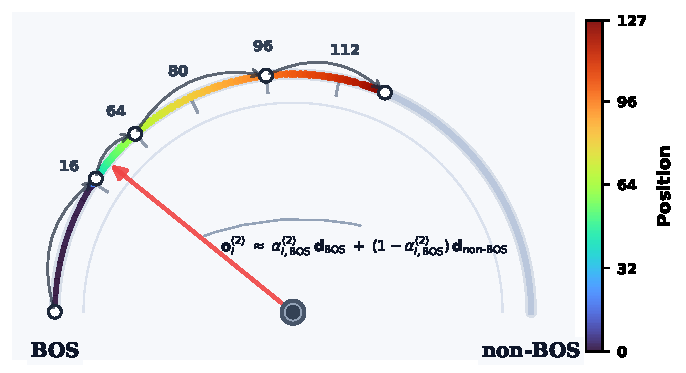
\includegraphics[width=0.95\columnwidth]{r0_directional_rotation_example.pdf}
\caption{\textbf{Directional trajectory (\modelfull, averaged).}
Layer-2 attention-output direction traces a smooth trajectory in the 2-D plane spanned by
$\{\dBOS{2}, \dNBOS{2}\}$. The trajectory is computed from mean attention-output vectors
over $n=64$ held-out sequences at $L=128$; for the full five-step mechanism and derivation,
see \Cref{sec:mechanism_text}.}
\label{fig:r0_gauge}
\vspace{-6mm}
\end{figure}

Transformers need token order.
In standard models, we give the network order explicitly using positional embeddings
(e.g., absolute, rotary, or bias-based schemes)~\citep{vaswani2017attention, wang2021rotary, alibi}.
In this paper we look at the extreme opposite setting:
we remove positional embeddings entirely and feed the model only token embeddings.
Surprisingly, prior work shows that an autoregressive (causal-masked) Transformer in this setting
(\textbf{NoPE}: no positional embeddings) can still recover \emph{absolute position}
(e.g., the model can tell whether a token is the 5th token or the 50th)~\citep{haviv2022transformer, kazemnejad2023lenghGeneralization}.
The basic puzzle is then: where does the index $i$ come from if we never feed $i$ into the model?

\paragraph{Why the common explanation is not the whole story.}
A natural place to look is the causal attention mask.
At position $i$, attention can only look at the prefix $0{:}i$.
That prefix gets longer as $i$ grows, so the attention output changes with $i$ even if the weights are the same.
Prior work makes this idea precise by showing a strong \emph{scale} / \emph{variance} trend:
if attention is close to uniform over the prefix, then the output is roughly an average of $(i{+}1)$ vectors,
so its variance shrinks with $i$~\citep{chi-etal-2023-latent}.
This is a real positional signal.

But most Transformers apply \emph{LayerNorm} throughout the network~\citep{ba2016layer}.
LayerNorm takes each token’s vector and rescales it to have (roughly) fixed magnitude.
So if we want a full end-to-end explanation of how position is decoded at the end of the network,
we cannot rely only on “the vector is larger/smaller at different positions”:
LayerNorm largely removes that information.
This raises the core question of this paper: \emph{after LayerNorm removes per-token scale, what remains that can still encode position?}

\paragraph{What is new here.}
Prior NoPE analyses characterize the prefix-averaging variance trend, but that signal alone is not an end-to-end explanation once LayerNorm is applied.
We give an end-to-end account of absolute-position encoding in a two-layer pre-norm NoPE Transformer after LayerNorm, and derive why the one-layer route is insufficient in our setting.
The mechanism has five steps. Layer 1 creates a shared \emph{BOS anchor} (\Cref{subsec:mech_step1}). The Layer-2 OV matrix (\Cref{subsec:preliminaries}) separates \bos and \nbos contributions into distinct directions (\Cref{subsec:mech_step2}). The \bos attention weight varies with position (\Cref{subsec:mech_step3}). The attention output interpolates between the two directions (\Cref{subsec:mech_step4}). A linear head decodes position (\Cref{subsec:mech_step5}).

\paragraph{The core idea: a shared anchor direction from \bos.}
We prepend a special beginning-of-sequence token, \bos, at position $0$.
This matters because in a causal model, every position $i>0$ can attend to position $0$.
So \bos is the one token that is guaranteed to appear in \emph{every} prefix.

Consider what Layer~1 attention produces under near-uniform weights.
When first-layer attention is approximately uniform over the causal prefix, it produces a weighted prefix average.
This is exactly the random-initialization regime analyzed in \Cref{app:1block_appendix}.
Because \bos is always inside that average, the first layer injects
a \emph{shared \bos-direction component} into the representation at \emph{every} position.
After the following LayerNorm, the length information is normalized away,
but this shared directional component persists.
This is the first crucial ingredient:
\textbf{the network gets a fixed reference direction that is shared across the whole sequence.}

This reference alone is noisy at the single-sequence level.
The mechanism described in \Cref{sec:mechanism_text} shows how the second layer can turn it into a clean per-position signal, and \Cref{sec:empirical} verifies that trained models do so.

\paragraph{How the second layer turns the anchor into a clean position code.}
The mechanism predicts that the second layer produces two directions and mixes them in a position-dependent way.

\textbf{(1) Two directions.}
Directional separation requires that the \bos and \nbos aggregate contributions point in distinct directions.
Directional coherence requires that the \nbos aggregate direction remains stable across positions.
\Cref{subsec:mech_step2} states these conditions formally, \Cref{sec:empirical} verifies them in trained models, and \Cref{sec:write_bottleneck} tests their causal role.

\textbf{(2) A BOS attention weight that changes with position.}
The mechanism requires that the \bos attention weight in Layer~2 varies with position.
A natural source is softmax normalization: as the prefix grows, more keys compete, so the \bos fraction decreases.
\Cref{sec:empirical} verifies this trend in trained models.
This position-dependent \bos attention weight controls the interpolation.

\textbf{(3) Directional trajectory.}
Putting (1) and (2) together:
at early positions the output is closer to the \bos-associated direction,
and at later positions it moves toward the \nbos direction.
Geometrically, the representation’s direction traces a smooth path between two directions as $i$ increases
(visualized in \Cref{fig:r0_gauge}).
A linear head can then read position from where the representation sits along that path.

The key point is that \textbf{usable position information is carried by direction, which survives LayerNorm.}

\paragraph{What we show empirically.}
We test this explanation in two training regimes: a controlled setting where the backbone is mostly frozen and only the second-layer attention and a linear head are trained, and a fully trained multi-head model.
In both cases, \Cref{sec:empirical} verifies the directional-separation and directional-coherence conditions required by the mechanism.

We also show that the position computation is effectively low-dimensional: keeping only two dominant directions of the second-layer attention update preserves almost all decoding performance. This is consistent with position as a one-parameter movement in the 2D plane spanned by the \bos and \nbos directions.

\paragraph{Contributions.}
We make four contributions. First, we derive the two-layer algebraic mechanism for absolute-position decoding after LayerNorm (\Cref{sec:mechanism_text}). Second, we verify in \modelminimal and \modelfull that trained models satisfy its required conditions (\Cref{sec:empirical}). Third, we provide causal verification through OV-subspace interventions (\Cref{sec:write_bottleneck}). Fourth, we show why the one-layer route is insufficient in our setting (\Cref{app:1layer_vs_2layer}).

\paragraph{Roadmap.}
\Cref{sec:mechanism_text} derives the mechanism. \Cref{sec:empirical} verifies that trained models satisfy the required conditions in two regimes (\modelminimal and \modelfull). \Cref{sec:write_bottleneck} provides causal validation via OV-subspace interventions. \Cref{app:1block_appendix} analyzes the one-layer case.

\section{Notation}
\label{sec:notation}
In this section, we define the architecture used throughout the paper: a two-layer pre-norm causal Transformer
\citep{vaswani2017attention, radford2019language, Baevski2018AdaptiveIR, Xiong2020OnLN} followed by a linear
regression head that predicts absolute token position.

\paragraph{Data.}
We consider sequences of length $n$ with tokens $t_0,\dots,t_{n-1}$, where $t_0$ is always the \bos (beginning-of-sequence) token.
Let $e_i \in \R^d$ denote the token embedding at position $i$.
We study the NoPE setting: the model receives only token embeddings (no positional embeddings).

\paragraph{Model: pre-norm causal Transformer.}
We study a two-layer, pre-norm, causal Transformer.
Let $h_i^{0} := e_i$ be the residual-stream state at position $i$ immediately after the token embedding.
Each layer $\ell\in\{1,2\}$ applies LayerNorm \emph{before} each sublayer (attention and MLP) and then adds the resulting update back
into the residual stream via a skip connection. We write the LayerNorm explicitly because our mechanism later hinges on which statistics
it removes (per-token mean/variance) and what it preserves (directional information after centering).

\paragraph{LayerNorm.}
For $u\in\R^d$, define
\begin{align}
&\LN(u) \;:=\; g \odot \frac{u - \mu(u)}{\sqrt{\sigma^2(u)+\varepsilon}} \;+\; b, \\
&\mu(u) \;=\;\frac{1}{d}\sum_{k=1}^d u_k,\qquad
\sigma^2(u)\;=\;\frac{1}{d}\sum_{k=1}^d (u_k-\mu(u))^2,
\end{align}
where $g,b\in\R^d$ are gain/bias parameters (learned or fixed) and $\varepsilon>0$ is a constant.

\paragraph{Layer equations (pre-norm form).}
Given the incoming residual $h_i^{\ell-1}$, the attention sublayer receives the normalized states
$x_i^{(\ell)} \defeq \LN(h_i^{\ell-1})$ and produces an attention update $o_i^{(\ell)}$ from the causal prefix.
This update is added into the residual stream, after which the MLP sublayer again sees a normalized version of the updated residual.
Concretely, for each position $i$:
\begin{align}
x_i^{(\ell)} &\defeq \LN\!\big(h_i^{\ell-1}\big), \label{eq:first_layer_norm} \\
o_i^{(\ell)} &:= \Attn^{(\ell)}\!\big(x_{0:i}^{(\ell)}\big)\in\R^d, \\
\tilde h_i^{(\ell)} &:= h_i^{\ell-1} + o_i^{(\ell)}, \\
m_i^{(\ell)} &:= \MLP^{(\ell)}\!\Big(\LN\!\big(\tilde h_i^{(\ell)}\big)\Big)\in\R^d, \\
h_i^{\ell} &:= \tilde h_i^{(\ell)} + m_i^{(\ell)}.
\end{align}
We denote by $h_i^{(1)}$ and $h_i^{(2)}$ the residual streams after Layers~1 and~2, respectively.
Our mechanistic analysis traces how position information propagates through these residual updates.

\paragraph{Causal self-attention.}
For a given layer $\ell$ and positions $i, j$, we always assume $0\le i \le n-1$ and $0\le j \le i$.
Moreover, we denote the query position as $i$ and the key/value positions as $j$.
\begin{align}
q_i^{(\ell)} &= W_Q^{(\ell)} x_i^{(\ell)} + b_Q^{(\ell)},\quad
k_j^{(\ell)} = W_K^{(\ell)} x_j^{(\ell)} + b_K^{(\ell)}, \\
v_j^{(\ell)} &= W_V^{(\ell)} x_j^{(\ell)} + b_V^{(\ell)},
\end{align}
with $W_Q^{(\ell)},W_K^{(\ell)},W_V^{(\ell)}\in\R^{d_h\times d}$ (and biases in $\R^{d_h}$).
Attention scores and weights are defined as
\begin{align}
s_{i,j}^{(\ell)} &= \frac{\big(q_i^{(\ell)}\big)^\top k_j^{(\ell)}}{\sqrt{d_h}},
\qquad
s_{i,j}^{(\ell)}=-\infty \;\;\text{for}\;\; j>i \;\; \\
\alpha_{i,j}^{(\ell)} &= \softmax_{j\le i}\!\big(s_{i,j}^{(\ell)}\big),
\qquad
\sum_{j\le i}\alpha_{i,j}^{(\ell)}=1,
\end{align}
and the (pre-output-projection) attention aggregation is
\begin{equation}
z_i^{(\ell)} = \sum_{j\le i}\alpha_{i,j}^{(\ell)} v_j^{(\ell)} \in \R^{d_h}.
\end{equation}
The attention update written into the residual stream is
\begin{equation}
\label{eq:attn_output}
o_i^{(\ell)} = W_O^{(\ell)} z_i^{(\ell)} + b_O^{(\ell)} \in \R^d,
\end{equation}
where $W_O^{(\ell)}\in\R^{d\times d_h}$ and $b_O^{(\ell)}\in\R^d$.
(For multi-head attention, $z_i^{(\ell)}$ is the concatenation of per-head $z_i^{(\ell,h)}$, $W_O^{(\ell)}$ is shared across heads,
and the definitions below hold with the \emph{fused} $W_V^{(\ell)}$ and $W_O^{(\ell)}$.)

The mechanism-specific quantities (the OV matrix, directional
definitions, and intervention tools) are introduced in
\Cref{subsec:preliminaries}.

\paragraph{Conventions.}
Indices $i,j$ denote \emph{positions}. Expectations $\E[\cdot]$ and variances $\Var(\cdot)$ are over tokens
from the evaluation set unless stated otherwise.
``\bos'' refers to position $0$, and ``\nbos'' refers to positions $j>0$.
For activation/attention symbols, superscripts written via $\lidx{\cdot}$ denote \emph{layer indices}, not powers
(e.g., $\oB{i}$ means Layer~2 attention update at position $i$).
When we mean squaring, we write it explicitly with parentheses, e.g., $(\oB{i})^2$.
 
\section{Background and Related Work}
%%%%%%%%%%%%%%%%%%%%%%%%%%%%%%%%%%%%%%%%%%%%%%%%%%%%%%%%%%%%%%%%%%%%%%%%%%%%%%%
\label{sec:background}
% \label{sec:variance}
We refer the reader to \Cref{sec:notation} for a complete description of our notation.%, and to \Cref{tab:notation} for quick reference.

\paragraph{Positional representations in Transformers.}
Most Transformer architectures inject positional information explicitly.
The original Transformer uses absolute positional encodings \citep{vaswani2017attention}, and later work introduced alternatives such as relative position representations \citep{shaw2018self}, rotary embeddings \citep{wang2021rotary}, and linear attention biases (ALiBi) for improved length extrapolation \citep{alibi}.
These methods encode order through explicit positional parameterization.

\paragraph{Implicit positional information without positional embeddings.}
Recent work shows that causal Transformers without positional embeddings (NoPE) can still represent absolute position \citep{haviv2022transformer}.
In particular, \citet{chi-etal-2023-latent} show that a position signal appears in self-attention output variance under causal prefix averaging.
Related analyses study the interaction between positional encoding choices and length generalization \citep{kazemnejad2023lenghGeneralization}, and emerging positional structure in NoPE via local embedding similarity \citep{zuo2025position}.
These findings establish that positional signals exist in NoPE, but they do not provide a complete end-to-end circuit through the full Transformer computation.

\paragraph{Mechanistic interpretability.}
Mechanistic interpretability seeks to reverse-engineer neural networks into interpretable computational components \citep{elhage2021mathematical, elhage2022toy}.
In this framework, \textbf{circuits} denote specific pathways of parameters and activations implementing a function, as demonstrated in prior analyses such as induction heads \citep{olsson2022context} and automated circuit discovery \citep{conmy2023towards}.
Our work uses this lens to identify and validate a complete positional-encoding circuit in NoPE Transformers.

\textbf{From variance to direction: reconciling with prior work.} We first summarize the variance-based account of
\citet{chi-etal-2023-latent}, then explain why it is incomplete under LayerNorm, and finally position our directional mechanism.

\textbf{Variance.} \citet{chi-etal-2023-latent}, in Lemma 3, identified variance of self-attention outputs as a signal that correlates with token position. Even under random initialization and in the absence of positional embeddings, the second moment of the attention outputs varies systematically across positions, scaling as $1/(i+1)$.

Using the notation in \Cref{sec:notation}, consider one attention head in layer $\ell$. If initialization keeps attention scores $s_{i,j}^{(\ell)}$ small, then after causal masking the softmax is approximately uniform over the prefix:
\begin{equation}
\alpha_{i,j}^{(\ell)} \approx
\begin{cases}
\frac{1}{i+1}, & j \le i, \\
0, & j > i.
\end{cases}
\label{eq:first_attn_output}
\end{equation}
Therefore, the pre-output attention aggregate is approximately
\[
z_i^{(\ell)} = \sum_{j\le i}\alpha_{i,j}^{(\ell)} v_j^{(\ell)}
\;\approx\;
\frac{1}{i+1}\sum_{j=0}^{i} v_j^{(\ell)}.
\]
If the value vectors are i.i.d.\ with per-coordinate variance $\sigma_v^2$, then each coordinate of $z_i^{(\ell)}$ has variance $\sigma_v^2/(i+1)$. This positional dependence of the second moment provides a signal that can be used to infer token position.\footnote{At initialization, $W_V$ is approximately orthogonal up to scale, so applying it to i.i.d. token features preserves the same $1/(i+1)$ scaling.}

\textbf{LayerNorm and why the variance explanation is incomplete.}
After the attention update is added through the residual connection, LayerNorm is applied.
LayerNorm is a standard component in Transformer architectures \citep{ba2016layer, Xiong2020OnLN}.
LayerNorm largely removes per-token scale, so the raw variance trend above cannot directly serve as the final decoding signal.

In Lemma 4, \cite{chi-etal-2023-latent} explicitly computes the post-LayerNorm variance (in their notation) as
\[
\frac{ m\sigma^2 + \sum_i \left( \mathbf{W}_{o,j:}\mathbf{W}_{v,:i} \right)^2 }
     { m\sigma^2 + d^2\sigma^4 },
\]
and the authors claim that ``as long as $\sum_i \left( \mathbf{W}_{o,j:}\mathbf{W}_{v,:i} \right)^2 \neq d^2 \sigma^4$, the classifier should be able to exploit the discrepancy to recover position.''

Yet this mechanism is likely weak in practice, because $\sum_i \left( \mathbf{W}_{o,j:}\mathbf{W}_{v,:i} \right)^2$ concentrates around its mean at initialization, leaving only a small discrepancy to exploit.

\textbf{Our perspective and what survives LayerNorm.}

In contrast to \citet{chi-etal-2023-latent}, which analyze the variance of representations at each token position, we adopt a different perspective. We show that a trained two-layer transformer can exploit explicit knowledge of the embedding vectors--specifically, their \emph{directions} in representation space--to recover token positions. Thus, while LayerNorm removes variance information, the directional information is preserved and remains accessible to the model.


\begin{figure*}[t]
\centering
\scalebox{0.92}{
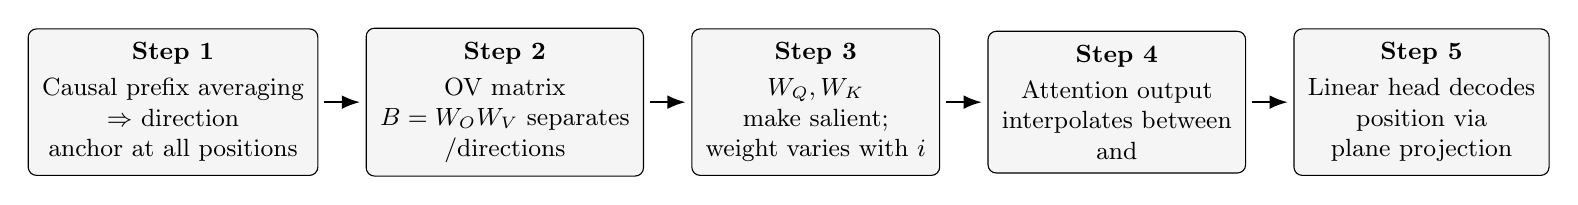
\begin{tikzpicture}[
  font=\small,
  >=Latex,
  node distance=4mm and 6mm,
  stepbox/.style={
    draw, rounded corners=3pt,
    fill=gray!8, align=center,
    inner sep=5pt, minimum width=2.8cm, minimum height=1.8cm
  },
  arr/.style={->, thick, shorten <=2pt, shorten >=2pt}
]

% Step 1
\node[stepbox] (s1) {
  \textbf{Step 1}\\[2pt]
  Causal prefix averaging\\
  $\Rightarrow$ \bos direction\\
  anchor at all positions
};

% Step 2
\node[stepbox, right=of s1] (s2) {
  \textbf{Step 2}\\[2pt]
  OV matrix\\
  $B=W_OW_V$ separates\\
  \bos/\nbos directions
};

% Step 3
\node[stepbox, right=of s2] (s3) {
  \textbf{Step 3}\\[2pt]
  $W_Q,W_K$\\
  make \bos salient;\\
  \bos weight varies with $i$
};

% Step 4
\node[stepbox, right=of s3] (s4) {
  \textbf{Step 4}\\[2pt]
  Attention output\\
  interpolates between\\
  \bos and \nbos
};

% Step 5
\node[stepbox, right=of s4] (s5) {
  \textbf{Step 5}\\[2pt]
  Linear head decodes\\
  position via\\
  plane projection
};

% Arrows
\draw[arr] (s1) -- (s2);
\draw[arr] (s2) -- (s3);
\draw[arr] (s3) -- (s4);
\draw[arr] (s4) -- (s5);


\end{tikzpicture}
}
% \vspace{-3mm}
\caption{\textbf{The five-step mechanism.} Step~1 injects a \bos-direction component into every position through causal prefix averaging (after the succeeding LayerNorm).
Step~2 uses the Layer-2 OV matrix $B=W_O^{(2)}W_V^{(2)}$ to separate \bos-indexed and \nbos directions.
Step~3 makes the \bos key salient, producing a position-dependent \bos attention weight $\alpha^{(2)}_{i,\mathrm{BOS}}$.
Step~4 turns this scalar into a smooth interpolation of the attention output between the \bos and \nbos directions as position increases.
Step~5 decodes that trajectory with a linear head that has nontrivial projection onto the plane $\mathrm{span}\{\dBOS{2}, \dNBOS{2}\}$.}
\label{fig:mechanism_overview}
\vspace{-5mm}
\end{figure*}

\section{The Mechanism: Position Encoding in a 2-Layer Transformer}
\label{sec:mechanism_text}
We describe a mechanism by which a two-layer NoPE
transformer can encode absolute position using only the causal
mask and the direction of the attention output in the residual stream,
making position linearly decodable.
\Cref{sec:empirical} tests whether trained models realize this mechanism.

A single-layer transformer does produce a positional signal:
projecting onto the \bos direction yields a component that scales
as $\Theta(d/\sqrt{i})$ with noise $O(\sqrt{d})$
(\Cref{app:1block_appendix}).
However, the signal-to-noise ratio degrades at later positions,
and decoding position from a $1/\sqrt{i}$ scalar requires
a nonlinear inversion that the remaining half of the MLP cannot
implement.\footnote{To extract the $\dBOS{1}$ signal, $W_1$ must align with the \bos direction, leaving only $W_2 \circ \mathrm{act}(\cdot)$ to map $s \mapsto 1/s^2$. This is a linear model over a fixed elementwise nonlinearity, effectively a scaled activation function, which cannot implement the required inversion. See \Cref{app:1layer_vs_2layer}.}
The two-layer mechanism below sidesteps both limitations:
it produces an approximately affine signal that a linear head suffices to decode.

The mechanism involves five steps.
Since LayerNorm removes magnitude information, position must be
encoded in \emph{direction} alone.
In the first layer, the causal mask ensures that every position
attends to \bos, so the attention output mixes \bos with the other
tokens in the prefix, injecting a shared directional component
into every position: the \emph{BOS anchor}.
In the second layer, a matrix multiplication maps this shared
component and the \nbos component to two separated directions.
The attention weight on \bos decreases with position, so the
second-layer output interpolates between these two directions:
early positions lie closer to one, late positions to the other.
A linear head reads off position from this directional signal.
\Cref{fig:mechanism_overview} summarizes the circuit,
and \Cref{fig:r0_gauge} visualizes the trajectory.


\subsection{Preliminaries}
\label{subsec:preliminaries}

We define below the quantities used by the five-step circuit.

\paragraph{OV matrix and affine form.}
Expanding $v_j^{(\ell)}$ in \Cref{eq:attn_output} gives
\begin{align}
o_i^{(\ell)}
&= \sum_{j\le i}\alpha_{i,j}^{(\ell)}\,
   \underbrace{W_O^{(\ell)} W_V^{(\ell)}}_{\defeq\, B^{(\ell)}\;\in\;\R^{d\times d}}
   x_j^{(\ell)}
   \;+\; \underbrace{W_O^{(\ell)} b_V^{(\ell)} + b_O^{(\ell)}}_{\defeq\, b_{\text{attn}}^{(\ell)}\;\in\;\R^d}.
\label{eq:attn_affine_ell}
\end{align}
The matrix $B^{(\ell)} \defeq W_O^{(\ell)} W_V^{(\ell)}$ is called the \emph{OV matrix} \citep{elhage2021mathematical}. It is the linear map from each input $x_j^{(\ell)}$ to its contribution $B x_j^{(\ell)}$ to the attention output.
\label{eq:def_B_ell}
Therefore, the attention update to the residual stream can be seen as an affine transformation.
The bias $b_{\text{attn}}^{(\ell)}$ is constant across positions and cannot by itself encode absolute position.

\paragraph{Layer-1 anchor directions.}
We first consider the representation immediately after Layer~1 attention and the succeeding LayerNorm:
\begin{equation}
\label{eq:step1_ln_h}
\bar h_i^{(1)} \;:=\; \LN\!\big(\tilde h_i^{(1)}\big).
\end{equation}
Define
\begin{equation}
\wBOS{1} \;:=\; \bar h_0^{(1)},
\qquad
\wNBOS{1} \;:=\; \E_{j>0}[\bar h_j^{(1)}],
\end{equation}
and normalized Layer~1 directions
\begin{equation}
\label{eq:d_bos_and_nonbos_ln1}
\dBOS{1} \;:=\; \frac{\wBOS{1}}{\|\wBOS{1}\|}, \quad
\dNBOS{1} \;:=\; \frac{\wNBOS{1}}{\|\wNBOS{1}\|}.
\end{equation}
These are used only in Step~1 analyses on $\bar h_i^{(1)}$.

\paragraph{Layer-2 OV directions (main mechanism).}
For Layer~2, the attention inputs are $x_i^{(2)} \defeq \LN(h_i^{(1)})$.
We abbreviate the Layer-2 OV matrix as
\begin{equation}
B \;:=\; B^{(2)} \;=\; W_O^{(2)}W_V^{(2)} \in \R^{d\times d}.
\end{equation}
Here $B$ is a \emph{weight matrix} (model parameters), while vectors of the form
$Bx_i^{(2)}$ are activations in its image (the OV subspace).
Define Layer~2 \bos/\nbos direction vectors
\begin{equation}
\wBOS{2} \;:=\; Bx_0^{(2)} \in \R^d,
\qquad
\wNBOS{2} \;:=\; \E_{j>0}[Bx_j^{(2)}] \in \R^d,
\end{equation}
and their normalized Layer~2 directions
\begin{equation}
\label{eq:d_bos_and_nonbos_l2}
\dBOS{2} \;:=\; \frac{\wBOS{2}}{\|\wBOS{2}\|},
\quad
\dNBOS{2} \;:=\; \frac{\wNBOS{2}}{\|\wNBOS{2}\|}.
\end{equation}

\paragraph{Linear readout head.}
We define the \emph{linear readout head} as
\begin{equation}
\hat y_i \;=\; w_{\text{head}}^\top h_i^{(2)} + b_{\text{head}},
\end{equation}
with $w_{\text{head}}\in\R^d$ and $b_{\text{head}}\in\R$.
We also use the analytic choice $w_{\text{head}}\propto \wNBOS{2}-\wBOS{2}$.

\subsection{The Five-Step Circuit}
\label{subsec:mechanism}

\paragraph{Step 1: Causal prefix averaging writes a \bos anchor into every position}
\label{subsec:mech_step1}

A sufficient condition for Step~1 is near-uniform Layer~1 attention over the causal prefix.
Under Xavier initialization, token embeddings are approximately orthogonal: for two independent embeddings $e_j,e_k$, standard concentration gives $|\cos(e_j,e_k)|=O(1/\sqrt{d})$ (\Cref{app:1block_appendix}).
After LayerNorm, QK scores between distinct tokens are $O(1/\sqrt{d})$.
After softmax over the causal prefix, these near-equal logits produce approximately uniform Layer-1 attention at initialization.
\Cref{sec:empirical} verifies that trained models satisfy it.
In particular, \bos receives weight $\approx 1/(i{+}1)$ at every query position~$i$.

Given this near-uniform attention, the Layer~1 output at position~$i$ is approximately the prefix average $\frac{1}{i+1}\sum_{j=0}^{i}e_j$.
The \bos embedding $e_0$ appears in every prefix and is identical across sequences, so it contributes a shared directional component to every position.
In contrast, each \nbos embedding $e_j$ ($j>0$) depends on the input token at that position and varies across sequences.
After the succeeding LayerNorm, per-token scale is removed but direction is preserved, so the normalized representation $\bar h_i^{(1)}$ (\Cref{eq:step1_ln_h}) retains a shared \bos-direction component $\dBOS{1}$ across positions, i.e.\ the \bos anchor.

\paragraph{Step 2: The OV matrix separates \bos and \nbos directions}
\label{subsec:mech_step2}
Step~1 injects the direction $\dBOS{1}$ into every input of Layer~2. 
Using the OV-matrix notation from \Cref{eq:attn_affine_ell}, the Layer~2 attention update can be written as
\begin{equation}
\oB{i} \;=\; \sum_{j\le i}\aBij{i}{j}\, B x_j^{(2)} \;+\; \battnB.
\label{eq:mech_step2_attnwrite}
\end{equation}
Each $x_j^{(2)}$ with $j>0$ has a nonzero \bos-direction component, inherited from Step~1.
Separating $j=0$ from $j>0$:
\begin{equation}
\oB{i}-\battnB
\;=\;
\alpha^{(2)}_{i,\mathrm{BOS}}\,\wBOS{2}
\;+
\sum_{j=1}^{i}\aBij{i}{j}\,B x_j^{(2)},
\label{eq:exact_index_mixture}
\end{equation}
For $i=0$, the sum is empty and \eqref{eq:exact_index_mixture} reduces to $\oB{0}-\battnB=\wBOS{2}$.
Since $\sum_{j=1}^{i}\alpha^{(2)}_{i,j}=1-\alpha^{(2)}_{i,\mathrm{BOS}}$, the second term is an attention-weighted aggregation of the \nbos tokens $\{Bx_j^{(2)}\}_{j=1}^{i}$.
The mechanism requires two conditions on the Layer-2 OV matrix:
(i)~\emph{directional separation}: $\dBOS{2}$ and $\dNBOS{2}$ are not parallel, so the two terms in~\eqref{eq:exact_index_mixture} point in distinct directions, and
(ii)~\emph{directional coherence}: the attention-weighted average $\sum_{j=1}^{i}\aBij{i}{j}\,Bx_j^{(2)}$ concentrates around a single direction $\dNBOS{2}$ across positions and sequences, so that $\oB{i}$ lies approximately in the two-dimensional subspace $\mathrm{span}\{\dBOS{2},\,\dNBOS{2}\}$.
\Cref{sec:empirical} verifies that trained models satisfy both conditions.
\Cref{sec:write_bottleneck} tests their causal role by interventions.

\paragraph{Step 3: The QK circuit creates a position-dependent \bos mixing coefficient}
\label{subsec:mech_step3}

The \emph{position-dependent scalar} that mixes the two directions in~\eqref{eq:exact_index_mixture} is the \bos attention weight $\alpha^{(2)}_{i,\mathrm{BOS}}$, which we call the \emph{mixing coefficient}.

\paragraph{\bos is made salient as a key.}
For the mixing coefficient to be large, the Layer-2 QK circuit must make \bos salient as a key: the \bos attention score $s_{i,0}^{(2)}$ must exceed typical \nbos scores $s_{i,j}^{(2)}$ for $j>0$.
Consequently, $\alpha^{(2)}_{i,\mathrm{BOS}}$ is large compared to a typical \nbos weight, so the term
$\sum_{j\le i}\aBij{i}{j} B x_j^{(2)}$ places substantial weight on the \bos-indexed direction $B x_0^{(2)}$.

\paragraph{Why $\alpha^{(2)}_{i,\mathrm{BOS}}$ decreases with position.}
Due to the causal mask, at query position $i$ the softmax normalizes only over keys in the prefix $j\le i$.
As $i$ increases, the number of \nbos keys in the prefix grows, increasing the softmax normalizer over $j\le i$.
The mechanism assumes the \bos score advantage $s_{i,0}^{(2)}$ does not grow enough with $i$ to offset this normalizer growth.
Under this assumption, $\alpha^{(2)}_{i,\mathrm{BOS}}$ decreases with $i$.
This gives the monotone position dependence used in Step~4.

\paragraph{Step 4: The Layer~2 attention output interpolates between the two directions}
\label{subsec:mech_step4}

Under the directional-coherence condition~(ii) from Step~2, the exact decomposition~\eqref{eq:exact_index_mixture} is well-approximated by a two-direction mixture:
\begin{equation}
\oB{i}
\;\approx\;
\alpha^{(2)}_{i,\mathrm{BOS}}\, \wBOS{2}
\;+\;
\big(1-\alpha^{(2)}_{i,\mathrm{BOS}}\big)\, \wNBOS{2}
\;+\;
\battnB.
\label{eq:two_dir_mixture_mech}
\end{equation}
As $i$ increases, $\alpha^{(2)}_{i,\mathrm{BOS}}$ decreases, so $\oB{i}$ moves continuously from the \bos direction toward the
\nbos direction.
The computation lives in the two-dimensional subspace $\mathrm{span}\{\wBOS{2},\wNBOS{2}\}$, but the position signal is one-dimensional: it is parameterized by the single scalar $\alpha^{(2)}_{i,\mathrm{BOS}}$ (\Cref{fig:r0_gauge}).

\paragraph{Linear readout.}
Substituting the analytic choice $w_{\text{head}} := \wNBOS{2}-\wBOS{2}$
into the projection of~\eqref{eq:exact_index_mixture} yields
\begin{equation}
\langle \oB{i}-\battnB,\,w_{\text{head}}\rangle
=
\underbrace{c_0\vphantom{\|\wNBOS{2}\|}}_{\text{bias}}
-
\underbrace{\alpha^{(2)}_{i,\mathrm{BOS}}}_{\substack{\text{QK} \\ \text{circuit}}}
\cdot
\underbrace{\|\wNBOS{2}-\wBOS{2}\|^2}_{\substack{\text{OV} \\ \text{circuit}}}
+ \epsilon_i,
\label{eq:head_projection_decomposition}
\end{equation}
where $c_0 := \langle \wNBOS{2},\, \wNBOS{2}-\wBOS{2}\rangle$ is
position-independent and
\[
\epsilon_i \;:=\; \Big\langle
\sum_{j=1}^{i}\alpha^{(2)}_{i,j} Bx_j^{(2)}
- \big(1-\alpha^{(2)}_{i,\mathrm{BOS}}\big)\wNBOS{2},\;
w_{\text{head}}
\Big\rangle
\]
is the residual from replacing the \nbos aggregate by its expected direction (directional coherence, Step~2).
The position signal decomposes into two contributions:
the \textbf{QK circuit} (Step~3) controls the mixing coefficient
$\alpha^{(2)}_{i,\mathrm{BOS}}$, which determines the \emph{schedule},
i.e., how the signal varies with position.
The \textbf{OV circuit} (Step~2) controls the slope
$\|\wNBOS{2}-\wBOS{2}\|^2$, which determines the
\emph{sensitivity}, i.e., how much signal each unit change in $\alpha^{(2)}_{i,\mathrm{BOS}}$
produces.
Expanding the slope:
\begin{align}
\|\wNBOS{2}-\wBOS{2}\|^2 \nonumber
&= \|\wBOS{2}\|^2 + \|\wNBOS{2}\|^2 \\
  &- 2\langle \wBOS{2},\wNBOS{2}\rangle.
\label{eq:slope_expansion}
\end{align}
This is maximized when $\langle \wBOS{2},\wNBOS{2}\rangle$ is most
negative, i.e., when $\dBOS{2}$ and $\dNBOS{2}$ are antipodal.
Antipodal OV directions therefore yield the steepest position signal
for a given $\alpha^{(2)}_{i,\mathrm{BOS}}$ schedule, making adjacent positions maximally
distinguishable.
\Cref{sec:empirical} tests whether trained models are near-antipodal in this sense.
If $\alpha^{(2)}_{i,\mathrm{BOS}}$ is monotone in $i$ (Step~3) and
$\epsilon_i$ stays small (directional coherence, Step~2), the projected
signal is monotone and high-quality.


\paragraph{Step 5: Reading the position signal from the residual stream}
\label{subsec:mech_step5}

The final residual stream after Layer~2 is
\begin{equation}
h_i^{(2)} \;=\; h_i^{(1)} + \oB{i} + \MLP^{(2)}\!\Big(\LN(h_i^{(1)} + \oB{i})\Big),
\end{equation}
and the model predicts position by
\begin{equation}
\hat y_i \;=\; w_{\text{head}}^\top h_i^{(2)} + b_{\text{head}}.
\end{equation}
Because the attention bias $\battnB$ (\Cref{eq:attn_affine_ell}) is constant in $i$, it can be absorbed into $b_{\text{head}}$ and does not affect the
position-dependent signal.
The necessary condition is $\langle w_{\text{head}},\, \wBOS{2}-\wNBOS{2}\rangle \neq 0$.
When this holds, and when $\alpha^{(2)}_{i,\mathrm{BOS}}$ is monotone in $i$ (Step~3) and Step~2 coherence holds, $\hat y_i$ varies monotonically with $\alpha^{(2)}_{i,\mathrm{BOS}}$ (\Cref{eq:head_projection_decomposition}).
When the OV directions are near-antipodal, $\wNBOS{2}-\wBOS{2}$ is approximately collinear with $\dNBOS{2}$, so aligning $w_{\text{head}}$ with either OV direction suffices.

\subsection{The position signal survives LayerNorm and the MLP}
\label{subsec:mech_implications}

LayerNorm normalizes per-token scale, so a pure scale-only code is not stable in this architecture.
The mechanism instead encodes position in the direction of the attention output.

\paragraph{The Layer-1 MLP need not destroy the \bos anchor.}
The Layer-2 input is $x_i^{(2)} = \LN(h_i^{(1)})$ where $h_i^{(1)} = e_i + o_i^{(1)} + m_i^{(1)}$ includes the Layer-1 MLP output $m_i^{(1)} = \MLP^{(1)}\!\big(\LN(\tilde h_i^{(1)})\big)$.
Under standard initialization (e.g. Xavier), both $o_i^{(1)}$ and $m_i^{(1)}$ have norms $O(\sqrt{d})$, so the MLP does not dominate the residual stream.
The attention output $o_i^{(1)}$ contains a systematic \bos-direction component shared across positions (Step~1).
A randomly initialized MLP has no preferred direction, and its projection onto $\dBOS{1}$ is $O(1)$ with no consistent sign.
The \bos-direction component in $h_i^{(1)}$ is therefore dominated by the attention contribution, and the \bos anchor survives into the Layer-2 input.

\paragraph{The Layer-2 MLP need not disrupt the readout.}
The Layer-2 MLP output $m_i^{(2)}$ adds $O(1)$ noise to $w_{\text{head}}^\top h_i^{(2)}$, while the interpolation signal from $\oB{i}$ has magnitude controlled by $\|\wNBOS{2}-\wBOS{2}\|^2$ (\Cref{eq:head_projection_decomposition}).
\Cref{sec:empirical} checks the practical impact.

%%%%%%%%%%%%%%%%%%%%%%%%%%%%%%%%%%%%%%%%%%%%%%%%%%%%%%%%%%%%%%%%%%%%%%%%%%%%%%%
\section{Empirical Evidence}
\label{sec:empirical}
%%%%%%%%%%%%%%%%%%%%%%%%%%%%%%%%%%%%%%%%%%%%%%%%%%%%%%%%%%%%%%%%%%%%%%%%%%%%%%%

We validate the mechanism in two complementary regimes.
First, in \Cref{subsec:minimal_evidence}, we study \modelminimal: a controlled two-layer NoPE Transformer in which only Layer~2 attention (single head) and the linear position head are trained, while all other components are frozen at random initialization.
This isolates the circuit and enables direct, step-by-step measurements.
Second, in \Cref{subsec:full_evidence}, we analyze \modelfull: a fully trained two-layer Transformer with 12 attention heads per layer.
Interestingly, despite greater capacity, \modelfull converges to the same \bos-anchored, two-direction geometry, demonstrating that the mechanism is learnable using gradient-based optimization in NoPE architectures.
For the one-layer baseline (\Cref{app:1_block_empirical}), training runs for 80K steps with attention frozen and only the MLP trainable.
Despite this extended training, the 1-layer model does not reach a robust positional encoding. While this confirms position information is extractable from the prefix-averaging output, the two-layer mechanism (\Cref{sec:mechanism_text}) provides a more robust solution that gradient descent reliably converges to.

\subsection{Experimental Setup}
\paragraph{Data and splits.}
We train and evaluate on sequences from OpenWebText \citep{openwebtext} with a \bos token prepended.
Training uses disjoint text sequences from validation; the target is absolute position $i\in\{0,\dots,L{-}1\}$ within each sequence.
Unless stated otherwise, models are trained at length $L=128$ and evaluated on held-out validation sequences at the same length.

\paragraph{Metric.}
We report coefficient of determination $R^2$ between predictions $\hat y_i$ and true positions $i$ over all tokens in the evaluated set.
% For length extrapolation curves, we additionally report squared Pearson correlation ($r^2$) between $\hat y_i$ and $i$ to factor out global affine rescaling.

\paragraph{Reporting convention.}
Diagnostics are computed on fixed held-out validation batches.
Final decoding and OV-intervention metrics are reported on fixed held-out evaluation sets of
$n_{\text{seq}}=1600$ sequences per model; the exact protocol is documented in \Cref{app:details}.

\paragraph{Models \& Training.}
% We evaluate on OpenWebText with BOS prepended and training length $L=128$.
We evaluate two model variants, both built on a two-layer pre-norm Transformer ($d=768$, no positional embeddings)
initialized with Xavier initialization \citep{glorot2010understanding}.
\modelminimal has one attention head per layer; all parameters are frozen except Layer~2 attention and the regression head.
% and Layer~2 trains attention plus a linear position head; the Layer~2 MLP and LayerNorm are frozen, and the head reads the full Layer~2 output.
\modelfull has 12 heads per layer and trains all parameters.
\modelminimal is trained for 40K steps and \modelfull for 20K steps.
We report best-checkpoint metrics for all models based on the regression validation MSE loss.

%%%%%%%%%%%%%%%%%%%%%%%%%%%%%%%%%%%%%%%%%%%%%%%%%%%%%%%%%%%%%%%%%%%%%%%%%%%%%%%
\subsection{\modelminimal: Validating the Mechanism in a Controlled Setting}
\label{subsec:minimal_evidence}
%%%%%%%%%%%%%%%%%%%%%%%%%%%%%%%%%%%%%%%%%%%%%%%%%%%%%%%%%%%%%%%%%%%%%%%%%%%%%%%

\modelminimal achieves strong position decoding with a single trainable attention head in Layer~2:
$R^2=0.991$ on 1,600 held-out sequences.
We now quantify each step of the mechanism.

\paragraph{Step 1: Causal prefix averaging writes a \bos anchor, but decoding is still incomplete.}
With Layer~1 frozen at random initialization, its attention remains near-uniform over the causal prefix (\Cref{fig:attn_maps_empirical}, left).
The mean entropy per query position is 3.77, close to the perfectly uniform baseline
\(\frac{1}{128}\sum_{t=0}^{127}\log(t+1)=3.878\) and far from a single-position distribution (entropy $0$).
Because each prefix always includes \bos, this aggregation injects a \bos-aligned component into every position.
After the succeeding LayerNorm, scale is normalized away but this directional anchor remains in $\bar h_i^{(1)}$
(\Cref{eq:step1_ln_h,app:1block_appendix,eq:app_bos_anchor_matrix,eq:d_bos_and_nonbos_ln1}).

\begin{figure}[H]
\centering
\begin{subfigure}{0.4\columnwidth}
\centering
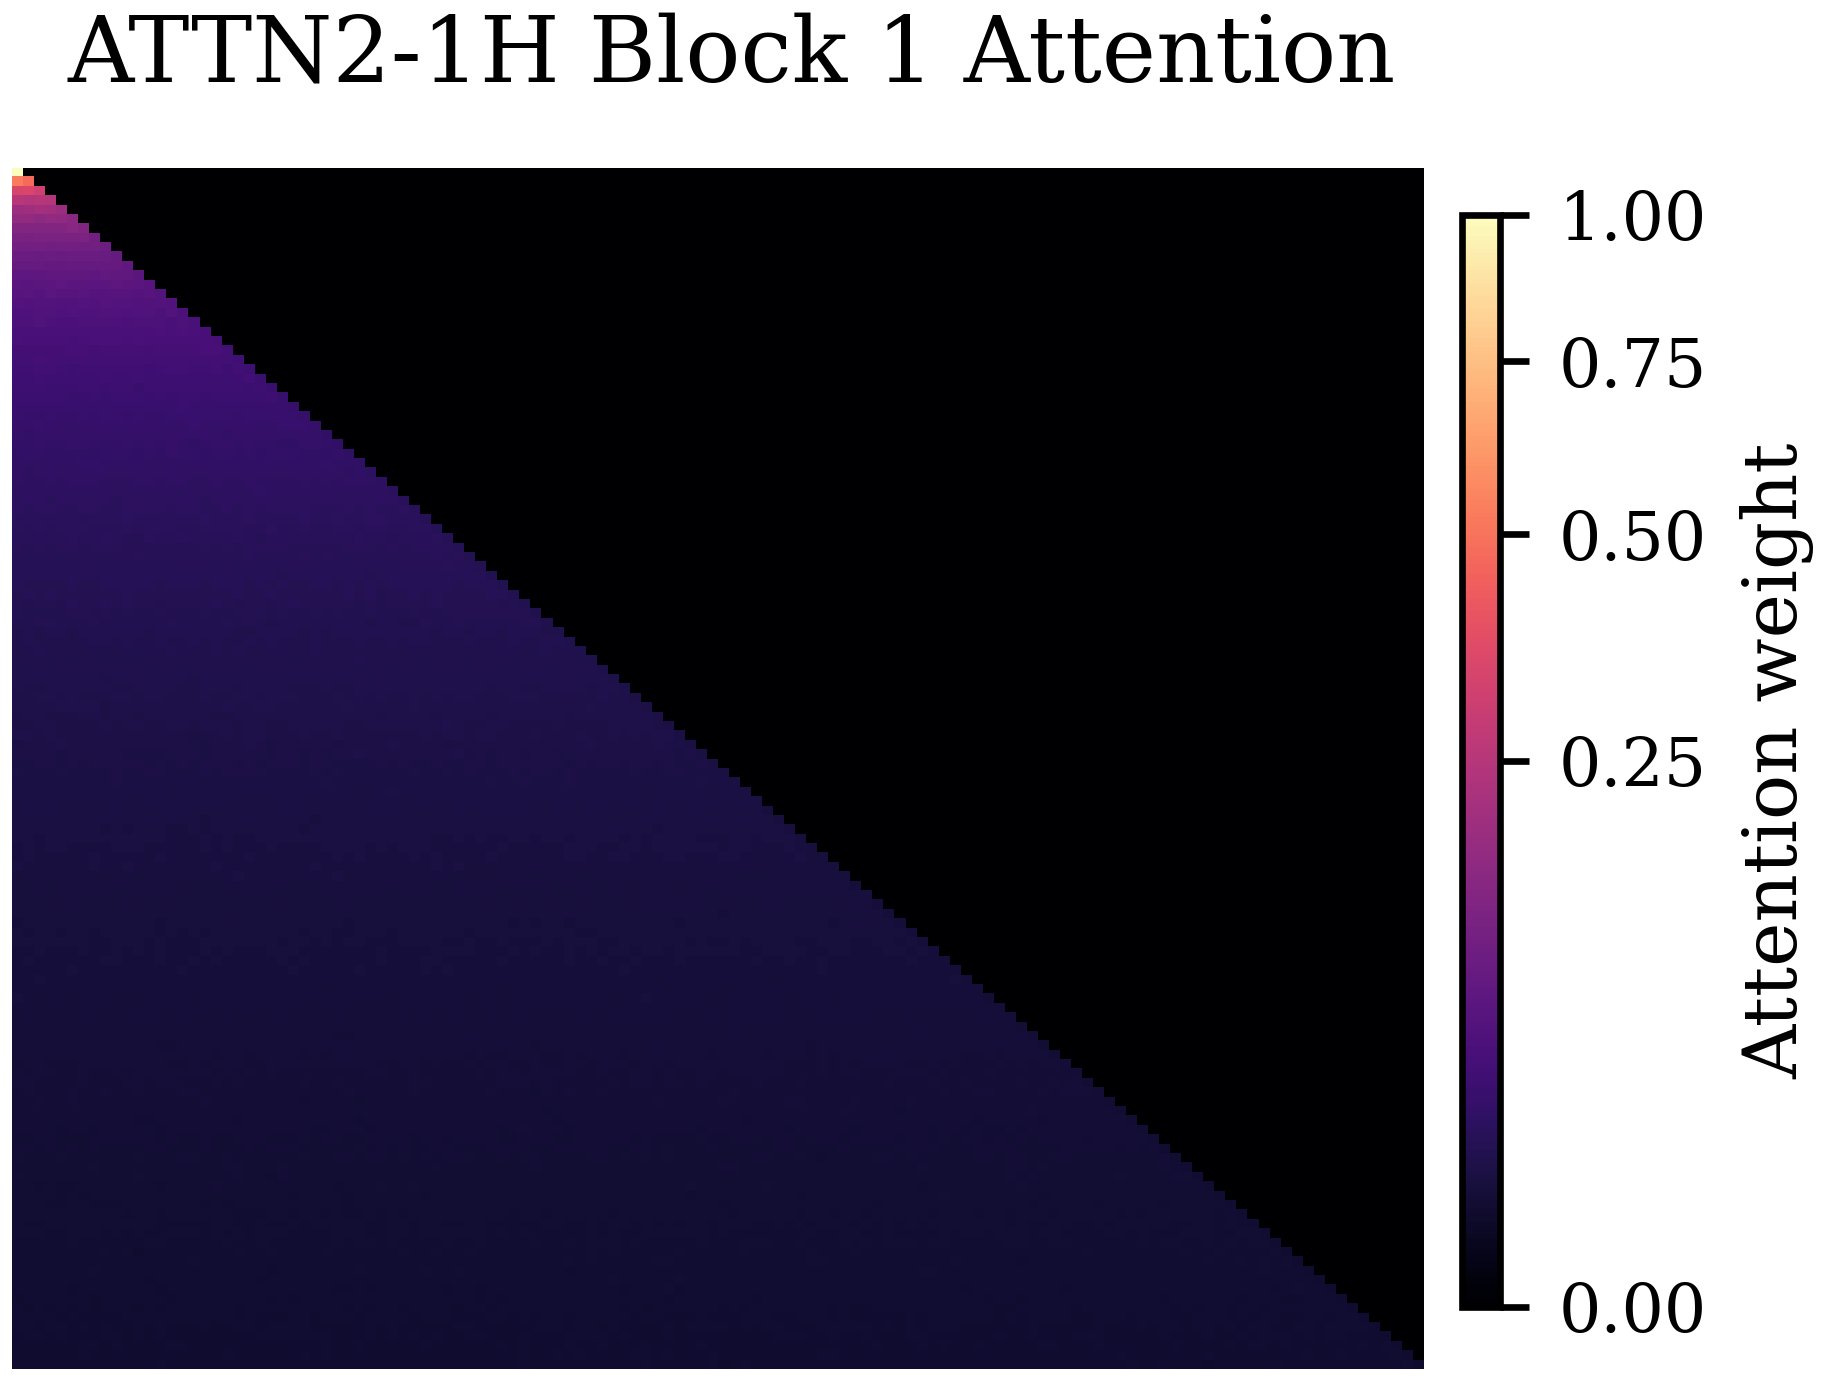
\includegraphics[width=\linewidth]{plots/attention_uniformity/attn2_1h_block1_attention.png}
\caption{\modelminimal 1st layer attention map.}
\end{subfigure}
\begin{subfigure}{0.4\columnwidth}
\centering
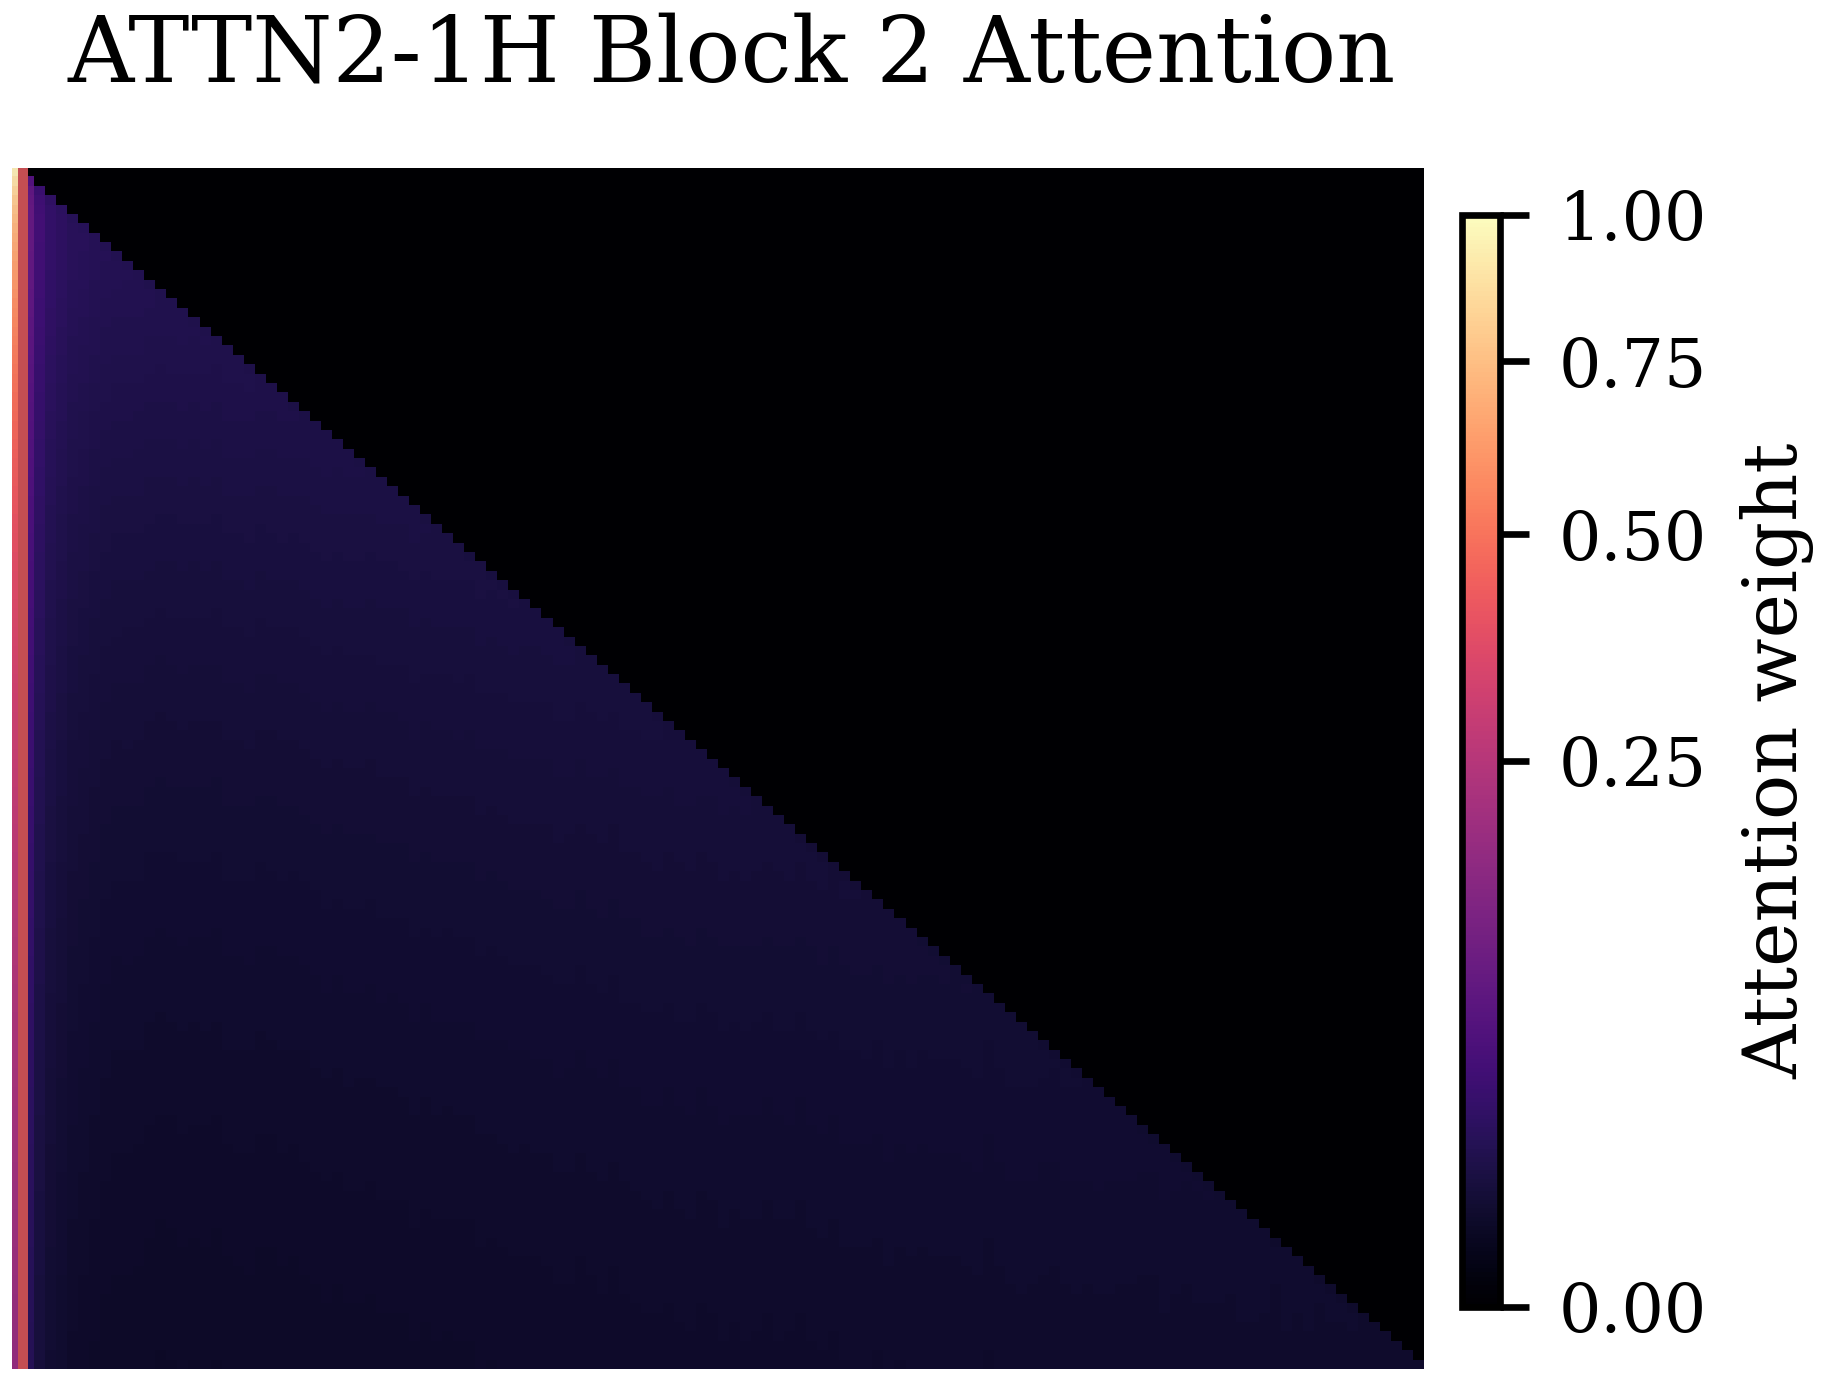
\includegraphics[width=\linewidth]{plots/attention_uniformity/attn2_1h_block2_attention.png}
\caption{\modelminimal 2nd layer attention map.}
% , BOS-attending ratio is $~22\times$.}
\end{subfigure}
\caption{\modelminimal \textbf{Attention maps.} Xavier initialization induces near-uniform Layer~1 attention,
while trained Layer~2 attention concentrates on \bos. Each map shows mean row-normalized attention
over held-out OpenWebText sequences at $L=128$.
The Layer~2 \bos-bias ratio is $r_h\approx22$ (\Cref{eq:bos_attention_metric}).}
\label{fig:attn_maps_empirical}
\vspace{-4mm}
\end{figure}

We then quantify what Step~1 alone already encodes in \modelminimal.
At the population level (position-wise means across sequences),
\(\rho_s(\E_b[\langle \bar h_i^{(1)}, \dBOS{1}\rangle], i)=-0.998\)
and
\(\rho_s(\E_b[\langle \bar h_i^{(1)}, \dNBOS{1}\rangle], i)=+0.999\).
However, at the individual-sequence level, median Spearman is much weaker:
$-0.647/+0.693$ (\bos/\nbos).
Thus, Step~1 shows a strong aggregate monotonic trend, but noisier sample-level structure (\Cref{fig:step1_projection_ln}).


\begin{figure}[H]
\centering
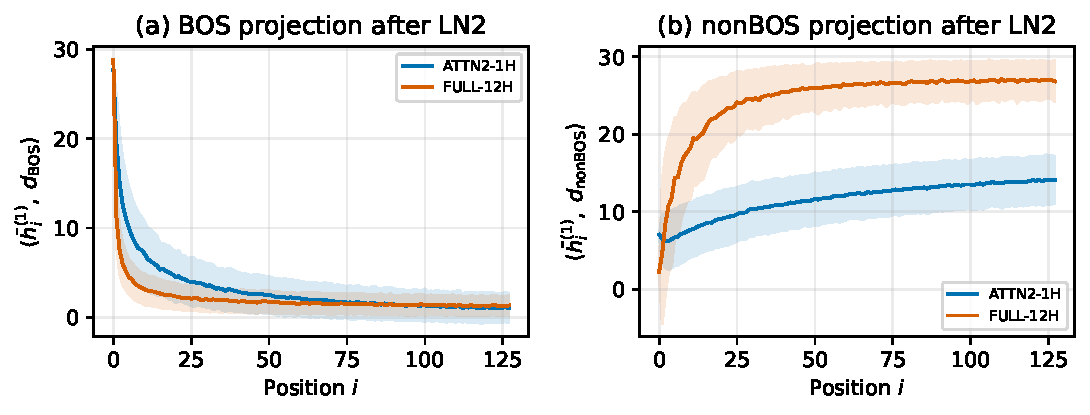
\includegraphics[width=1.0\columnwidth]{plots/bos_anchor_decodability_after_ln.pdf}
\caption{\textbf{Step~1 projections after the succeeding LayerNorm (Layer~1 LN2).}
Mean $\pm$ one standard deviation over held-out OpenWebText tokens for
$\langle \bar h_i^{(1)}, \dBOS{1}\rangle$ (left) and
$\langle \bar h_i^{(1)}, \dNBOS{1}\rangle$ (right).
Curves are computed from 10 batches of 64 sequences per model ($n_{\text{seq}}=640$).
Population-level trends are nearly monotonic; single-sequence trends are significantly weaker.
Position is only weakly linear decodable at this stage.}
\label{fig:step1_projection_ln}
\vspace{-3mm}
\end{figure}

Allowing a full linear probe on $\bar h_i^{(1)}$ still does not recover final decoding quality:
$R^2=0.543$.
This remains far below final model performance ($R^2=0.991$), showing that Step~1 provides only an anchor.
Full-model Step~1 statistics are reported in \Cref{subsec:full_evidence}.

\paragraph{Step 2: The OV matrix amplifies and separates \bos vs.\ \nbos directions.}
Layer~2 converts this structural \bos anchor into a directional signal via the OV matrix $B=W_O W_V$.
Although the input to this layer has already passed LayerNorm (per-token zero mean and unit variance), the OV matrix applies larger gain along the \bos direction than along typical \nbos directions.
In \Cref{eq:mech_step2_attnwrite}, the multiplication by $B$ strongly amplifies \bos's norm and maps \bos and \nbos to opposite directions, defined by $\dBOS{2}$ and $\dNBOS{2}$ (\Cref{eq:d_bos_and_nonbos_l2}) respectively.
Hence, the scalar products are:
\[
\|W_O v_{\text{BOS}}\|=394.9
\quad\text{vs.}\quad
\|W_O v_{\text{nonBOS}}\|=89.8
\quad (4.40\times),
\]
and the empirical \bos and \nbos directions are anti-correlated,
$\cos(\dBOS{2}, \dNBOS{2})=-0.660.$
This directional separation sets up a two-direction geometry in which attention can encode position via a mixing coefficient.

\paragraph{Step 3: Learned attention over-weights \bos.}
Layer~2 query/key projections make \bos salient as a key, producing a large \bos mixing coefficient (\Cref{fig:attn_maps_empirical}, Right).
To quantify \bos preference at the \emph{head} level, we use the following \bos-bias ratio (and report the per-head values in \Cref{tab:block2_bos_ratio}):
Let $a^{(2)}_{b,h}(t,j)$ denote the attention weight in Layer~2, head $h$, for sequence $b$, query position $t$, and key position $j$.
We use the shorthand $a^{(2)}_{b,h}(t,\bos) \defeq a^{(2)}_{b,h}(t,0)$ and define
\begin{align}
\label{eq:bos_attention_metric}
&r_h \;:=\;
\frac{\E_{b,\,t>0}\!\big[a^{(2)}_{b,h}(t,\bos)\big]}
{\E_{b,\,t>0}\!\big[\;\overline{a}^{(2)}_{b,h}(t,\nbos)\big]},
\\
&\overline{a}^{(2)}_{b,h}(t,\nbos) \;:=\; \frac{1}{t}\sum_{j=1}^{t} a^{(2)}_{b,h}(t,j).
\end{align}

$r_h$ is the average attention weight assigned to \bos divided by the average weight assigned to a \nbos key.
For \modelminimal (single head), this gives $r_h=21.9$ ($\approx 22\times$), i.e., \bos receives about 22 times more weight than a typical \nbos key.
Using the same held-out size declared in \Cref{sec:empirical} ($n_{\text{seq}}=1600$), the mean \bos-weight curve
\(\E_b[a^{(2)}_{b,0}(t,\bos)]\) decreases monotonically with position
(Spearman $=-1.0$).
This learned salience supplies the position-dependent scalar $\alpha^{(2)}_{i,\mathrm{BOS}}$ that drives the Step~4 interpolation.

\paragraph{Step 4: Attention output interpolates between two stable directions.}
As the \bos mixing coefficient varies with position, the Layer~2 attention output traces a smooth trajectory in the plane spanned by the \bos and \nbos directions.
Quantitatively, directional projections correlate strongly and with opposite signs.
At the population mean-curve level (average over sequences at each position),
\begin{align*}
&\mathrm{Spearman}(\oB{t}\!\cdot\! \dBOS{2},\, t)=-1,\\
&\mathrm{Spearman}(\oB{t}\!\cdot\! \dNBOS{2},\, t)=+1,
\end{align*}
while at the individual-sequence level, median per-sequence Spearman is
$-0.999/+0.999$ (\bos/\nbos) as seen in \Cref{fig:geom_gauge_proj_minimal}.
Compared with Step~1 sample-level Spearman ($-0.647/+0.693$),
this near-perfect monotonicity shows where sample-level decodability is gained.
The improvement follows directly from Steps~2--4: Step~2 applies the OV matrix $B=W_O W_V$ and creates two separated directions
($\wBOS{2},\wNBOS{2}$), Step~3 learns a position-dependent \bos coefficient $\alpha^{(2)}_{i,\mathrm{BOS}}$, and Step~4 computes
\(\oB{i} \approx \alpha^{(2)}_{i,\mathrm{BOS}} \wBOS{2} + (1-\alpha^{(2)}_{i,\mathrm{BOS}}) \wNBOS{2} + b\).
This one-parameter two-direction trajectory makes the signal linearly readable per sequence; along the difference axis $(\wNBOS{2}-\wBOS{2})$, \Cref{eq:head_projection_decomposition} predicts an affine trend in $\alpha^{(2)}_{i,\mathrm{BOS}}$ plus a residual \nbos aggregation term.
This is visualized in \Cref{fig:r0_gauge}.

To test the readout axis choice, we also project onto
$d_{\Delta}:=(\wNBOS{2}-\wBOS{2})/\|\wNBOS{2}-\wBOS{2}\|$.
In \modelminimal, both axes are monotone (mean-curve Spearman $=1.0$), but they are not equivalent:
$\cos(\dNBOS{2},d_{\Delta})=0.764$ (angle $40.2^\circ$), as shown in
\Cref{fig:axis_compare_main}.

\paragraph{Step 5: Linear head reads the interpolation.}
The learned linear head aligns with the $\dNBOS{2}$ direction:
\[
\cos(w_{\text{head}}, \dNBOS{2})=0.731.
\]
It is much less aligned with the difference axis,
$\cos(w_{\text{head}}, d_{\Delta})=0.154$,
showing that in \modelminimal the learned readout prefers $\dNBOS{2}$ over $d_{\Delta}$.
This matches the theory: choosing $w_{\text{head}}\propto (\wNBOS{2}-\wBOS{2})$ is sufficient, but not the unique optimum.
Analogously, we can interpret this convergence as an \emph{angular readout}: since the Layer~2 attention update $\oB{i}$ is well-approximated by a weighted mixture of the \bos and \nbos OV directions in a 2-D plane, the head effectively decodes position by mapping the mixture's angle in $\mathrm{span}\{\dBOS{2}, \dNBOS{2}\}$ to a scalar coordinate. Together, Steps 2--5 convert the causal \bos advantage into a directional form that is linearly readable at the output.


\begin{figure}[t]
\centering
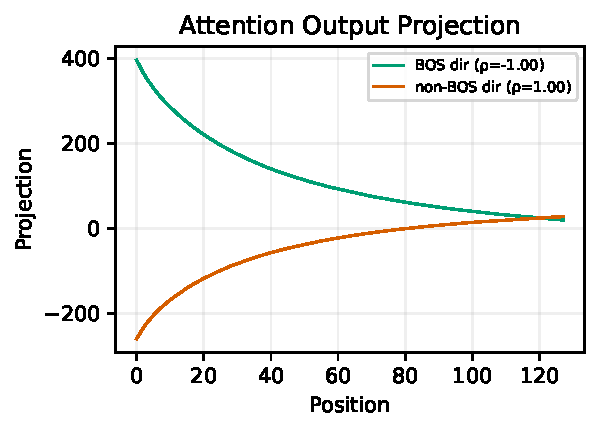
\includegraphics[width=0.92\columnwidth]{plots/r0_attention_output_projection/attention_output_projection_attn2_1h.pdf}
\caption{\textbf{Directional projections (\modelminimal).}
Mean projection curves of $\oB{t}$ onto $\dBOS{2}$ and $\dNBOS{2}$
over $n_{\text{seq}}=320$ held-out sequences at $L=128$; sample-level median Spearman is
$-0.999$ and $+0.999$ on $n_{\text{seq}}=320$ held-out sequences.}
\label{fig:geom_gauge_proj_minimal}
\vspace{-5mm}
\end{figure}

%%%%%%%%%%%%%%%%%%%%%%%%%%%%%%%%%%%%%%%%%%%%%%%%%%%%%%%%%%%%%%%%%%%%%%%%%%%%%%%
\subsection{\modelfull: Convergence to the Same Mechanism Under Full Training}
\label{subsec:full_evidence}
%%%%%%%%%%%%%%%%%%%%%%%%%%%%%%%%%%%%%%%%%%%%%%%%%%%%%%%%%%%%%%%%%%%%%%%%%%%%%%%

\modelfull attains near-perfect position decoding ($R^2=0.999$ on 1,600 held-out sequences)
and exhibits the same \bos-anchored two-direction geometry as \modelminimal.
Rather than repeating the step-by-step analysis, we highlight the \emph{differences} that arise under full training and use the trajectory visualization (\Cref{fig:r0_gauge}) as the main summary.
Complete quantitative diagnostics for Steps~1--5 (per-head statistics, attention maps, and projection curves) appear in \Cref{app:full_evidence_app}.

\paragraph{Same qualitative mechanism, with stronger two-direction geometry.}
Under full training, the effective OV subspace is still well-approximated by two stable directions aligned with
$\dBOS{2}$ and $\dNBOS{2}$, but the separation is cleaner than in \modelminimal
(e.g., $\cos(\dBOS{2},\dNBOS{2})\approx -0.97$; see \Cref{fig:gauge_projections_full}).
This sharper two-direction structure makes the downstream interpolation easier to visualize and measure.

\paragraph{Multiple heads implement \bos salience.}
Unlike \modelminimal (single trained head), \modelfull distributes the \bos preference across several Layer~2 heads.
We report the per-head \bos-bias ratios $r_h$ in \Cref{tab:block2_bos_ratio}; several heads strongly over-attend to \bos,
e.g., $r_h=100.3$ (H7), $76.5$ (H5), $62.6$ (H11), and $33.3$ (H10), while others are weak or near zero.
For these \bos-heavy heads, the mean \bos-weight curve also declines monotonically with position on
$n_{\text{seq}}=1600$ held-out sequences:
\(\rho_s(\E_b[a^{(2)}_{b,h}(t,\bos)],t)=-1.0\) for $h\in\{7,5,11,10\}$,
confirming monotone \bos decay in the strongest \bos-salient heads.
This heterogeneous profile still yields a robust aggregate \bos salience for the downstream mixture mechanism.

\paragraph{Trajectory visualization: smooth \bos-to-\nbos interpolation across positions.}
To summarize the mechanism in \modelfull, we visualize the Layer~2 attention output direction as interpolation between
$\dBOS{2}$ and $\dNBOS{2}$ (\Cref{fig:r0_gauge}).
As position increases, the direction advances smoothly from the \bos endpoint toward the \nbos endpoint, consistent with a
monotone decrease in the \bos mixing coefficient $\alpha^{(2)}_{i,\mathrm{BOS}}$.
Per-sequence trajectories (showing the effect holds at the individual-sequence level) are provided in \Cref{app:gauge_grid}.

\paragraph{Axis comparison: when \nbos and difference axes coincide.}
\Cref{fig:axis_compare_main} compares projection onto $\dNBOS{2}$ and onto
$d_{\Delta}:=(\wNBOS{2}-\wBOS{2})/\|\wNBOS{2}-\wBOS{2}\|$ in both models.
In \modelfull, these axes are nearly identical:
$\cos(\dNBOS{2},d_{\Delta})=0.984$ (angle $10.2^\circ$),
so both projections are practically equivalent.
Together with $\cos(\dBOS{2},\dNBOS{2})\approx -0.97$, this places \modelfull close to the antipodal regime from Section~4, where \nbos-aligned and difference-axis readouts become effectively the same at the attention-output level.
In \modelminimal, the same cosine is $0.764$ (angle $40.2^\circ$), so the two projections are distinct despite both being monotone.

\begin{figure}[t]
\centering
\begin{subfigure}{0.48\columnwidth}
\centering
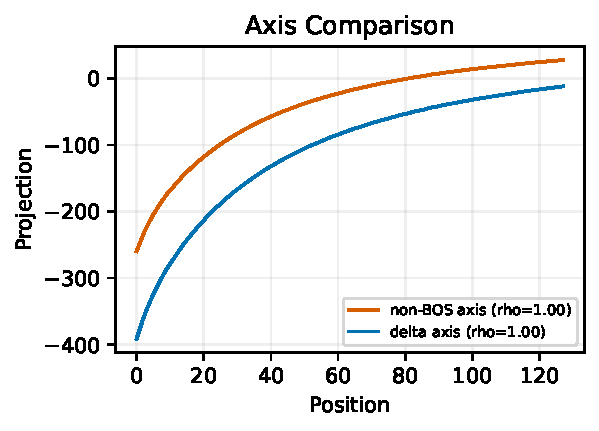
\includegraphics[width=\linewidth]{plots/r0_attention_output_projection/attention_output_axis_compare_attn2_1h.pdf}
\caption{\modelminimal}
\end{subfigure}
\hfill
\begin{subfigure}{0.48\columnwidth}
\centering
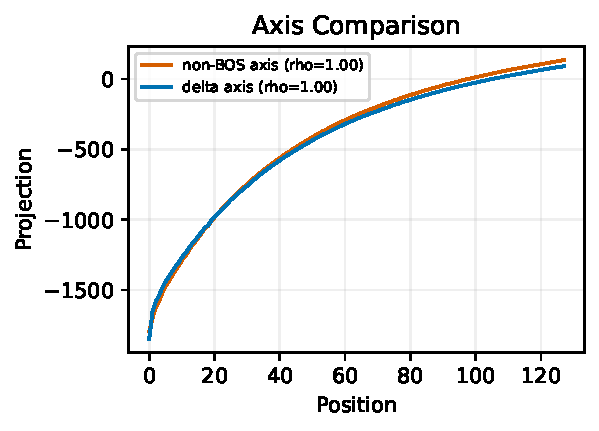
\includegraphics[width=\linewidth]{plots/r0_attention_output_projection/attention_output_axis_compare_full12h.pdf}
\caption{\modelfull}
\end{subfigure}
\caption{\textbf{Axis-comparison projections.}
Mean projection curves of $\oB{t}$ onto $\dNBOS{2}$ and
$d_{\Delta}=(\wNBOS{2}-\wBOS{2})/\|\wNBOS{2}-\wBOS{2}\|$ at $L=128$.
In \modelfull the two axes are nearly equivalent ($\cos=0.984$), while in \modelminimal they are more separated ($\cos=0.764$).}
\label{fig:axis_compare_main}
\vspace{-3mm}
\end{figure}

\paragraph{Residual cancellation and directional coherence.}
To validate the directional-coherence condition~(ii) from Step~2, we directly evaluate the residual term in
\Cref{eq:head_projection_decomposition}.
Define
\(
\Delta := \wNBOS{2}-\wBOS{2}
\)
and the projected residual term
\(
\langle \sum_{j=1}^{i}\alpha^{(2)}_{i,j} Bx_j^{(2)}
- (1-\alpha^{(2)}_{i,\mathrm{BOS}})\wNBOS{2},\,\Delta\rangle/\|\Delta\|^2
\).
This quantity is exactly the last term in \Cref{eq:head_projection_decomposition}, normalized by $\|\Delta\|^2$.
Empirically, it stays close to zero in both models (mean absolute value: $0.046$ for \modelminimal and $0.022$ for \modelfull), indicating strong cancellation of \nbos aggregation noise in this projection.
For concentration itself, the mean cosine between the normalized \nbos aggregate and $\wNBOS{2}$ over positions $i\ge16$ is $0.899$ (\modelminimal) and $0.938$ (\modelfull), consistent with the directional-coherence condition.



\paragraph{Step~1 remains incomplete; Layer~2 completes sample-level decodability.}
For \modelfull, Step~1 at $\bar h_i^{(1)}$ shows a population trend but weak sample-level monotonicity:
\(\rho_s(\E_b[\langle \bar h_i^{(1)}, \dBOS{1}\rangle], i)=-0.986\),
\(\rho_s(\E_b[\langle \bar h_i^{(1)}, \dNBOS{1}\rangle], i)=+0.981\), and median per-sequence Spearman
$-0.402/+0.486$ (\bos/\nbos).
A full linear probe on Step~1 reaches only $R^2=0.556$, far below final decoding.
After the Layer~2 computation of Steps~2--4 (OV-direction separation by $B$, learned \bos coefficient $\alpha^{(2)}_{i,\mathrm{BOS}}$,
and two-direction mixture in $\oB{i}$), per-sequence projection Spearman becomes
$-0.999/+0.999$,
showing that Layer~2 transforms the Step~1 anchor into a sample-level decodable signal.

\paragraph{Readout differs: weaker head alignment due to additional pathways.}
The regression head remains aligned with the \nbos direction but less strongly than in \modelminimal
(e.g., $\cos(w_{\text{head}},\dNBOS{2})=0.320$ and
$\cos(w_{\text{head}},d_{\Delta})=0.201$).
A natural explanation is that, in \modelfull, the trained Layer~2 MLP can also contribute position information, so the
linear head need not rely as directly on the pure attention-interpolation signal.
Again, this is consistent with Section~4: alignment to $d_{\Delta}$ is sufficient for decoding but not required.

\paragraph{Takeaway.}
Despite full parameter freedom and multi-head capacity, \modelfull converges to the same \bos-anchored mechanism
identified in \modelminimal; the trajectory in \Cref{fig:r0_gauge} provides a compact main-text summary, with full step-wise
measurements deferred to \Cref{app:full_evidence_app}.

%%%%%%%%%%%%%%%%%%%%%%%%%%%%%%%%%%%%%%%%%%%%%%%%%%%%%%%%%%%%%%%%%%%%%%%%%%%%%%%
\section{Validating the Mechanism}
\label{sec:write_bottleneck}
%%%%%%%%%%%%%%%%%%%%%%%%%%%%%%%%%%%%%%%%%%%%%%%%%%%%%%%%%%%%%%%%%%%%%%%%%%%%%%%
To validate that position information flows through a low-dimensional OV subspace,
we perform a causal intervention on the Layer~2 attention update.
\paragraph{OV-subspace intervention.}
Let $B = U\Sigma V^\top$ be the SVD decomposition of the OV matrix.
We define the rank-$r$ projector as $P_r := U_{1:r}U_{1:r}^\top$.
We define two interventions on the Layer~2 attention update $o_i$: \textit{retention} and \textit{ablation}:
\begin{align}
\tilde o_i &:= P_r\, o_i \quad \text{(retain top-$r$ directions)} \\
\tilde o_i &:= (I-P_r)\, o_i \quad \text{(ablate top-$r$ directions)}.
\end{align}
Retention \textit{keeps} the top-$r$ directions of the OV matrix, while ablation \textit{removes} the top-$r$ directions.
\paragraph{Intervened forward pass.}
We replace the attention update in the Layer~2 residual stream:
\begin{align}
\tilde h_i^{(2)} &:= h_i^{(1)} + \tilde o_i,
\end{align}
All other computations (LayerNorms, MLP, and the position head) are unchanged.
We evaluate $R^2$ between predicted and true positions on $n=1600$ sequences.


\paragraph{Results: \modelminimal.}
Using 1,600 held-out sequences, baseline decoding is $R^2=0.990$.
Retention of the top-1 singular direction yields $R^2=0.809$,
while top-2 retention recovers $R^2=0.991$, matching baseline performance.
When ablating the top-1 direction, performance drops to $R^2=0.125$.
Taken together, these results indicate that two dominant OV directions are sufficient for position decoding in \modelminimal.
\paragraph{Results: \modelfull.}
We observe similar trends with the second model.
Without intervention, \modelfull achieves $R^2=0.999$.
Retaining the top-1 and top-2 singular directions yields
$R^2=0.460$ and $R^2=0.951$, respectively.
Top-1 ablation drops performance to $R^2=0.625$.

\begin{figure}[t]
\centering
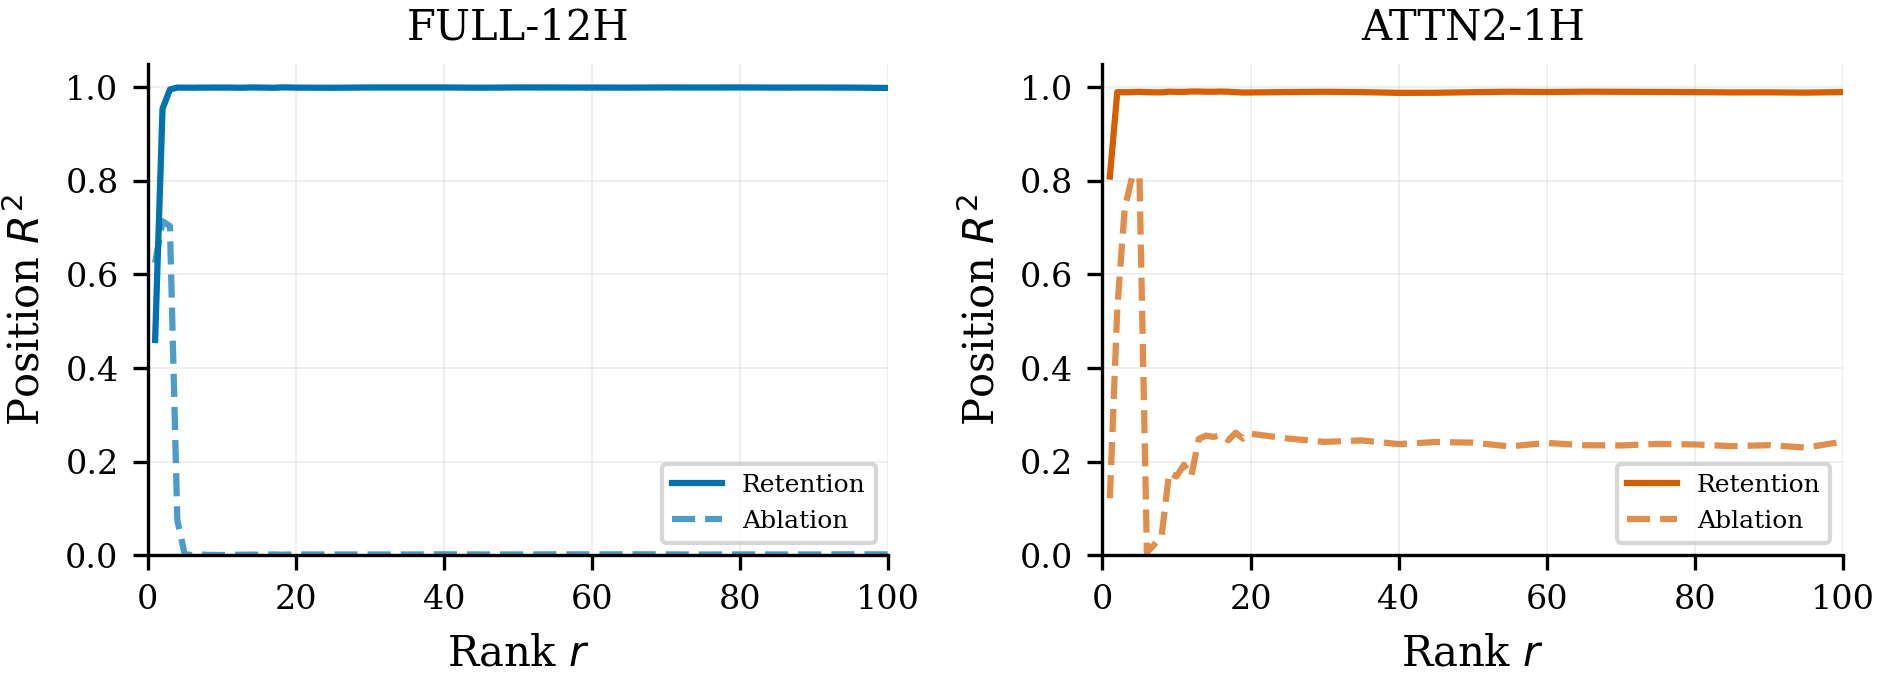
\includegraphics[width=1.\columnwidth]{plots/write_bottleneck_curves_all.png}
\caption{\textbf{OV-subspace bottleneck.}
Position decoding is recovered with only two singular vectors of the OV matrix $B$.
Solid lines: retention ($\tilde o_i=P_r o_i$). Dashed lines: ablation ($\tilde o_i=(I-P_r)o_i$).
Curves use held-out OpenWebText sequences; textual statistics are computed on held-out sets of $n_{\text{seq}}=1600$ sequences per model.
Both \modelminimal (ATTN2-1H) and \modelfull (FULL-12H) exhibit a low-rank bottleneck.}
\label{fig:write_bottleneck}
\vspace{-5mm}
\end{figure}
Intervention results presented in \Cref{fig:write_bottleneck}.

% \section{Conclusions}

%%%%%%%%%%%%%%%%%%%%%%%%%%%%%%%%%%%%%%%%%%%%%%%%%%%%%%%%%%%%%%%%%%%%%%%%%%%%%%%
\section{Conclusions}
%%%%%%%%%%%%%%%%%%%%%%%%%%%%%%%%%%%%%%%%%%%%%%%%%%%%%%%%%%%%%%%%%%%%%%%%%%%%%%%

The mechanism gives a complete circuit-level account of position encoding in NoPE Transformers.
Step~1 provides a \bos-direction component after LayerNorm; Steps~2--4 convert that component into a two-direction OV-subspace trajectory with near-perfect per-sequence monotonicity; and Step~5 reads this trajectory linearly.

To our knowledge, this is the first full end-to-end mechanism for positional encoding through the full Transformer computation, rather than an analysis restricted to attention-output statistics.
The same mechanism appears in two complementary regimes, a mostly random-initialized frozen-backbone model and a fully trained multi-head model, showing that it is robust and a natural outcome of gradient-based optimization.

The mechanism is also causally validated: OV-subspace interventions show that retaining only the top two singular OV directions recovers most decoding performance in both \modelminimal and \modelfull.
Relative to prior variance-based analyses~\citep{chi-etal-2023-latent}, this explains \emph{how} positional information remains usable after LayerNorm: the robust signal is directional rather than purely norm-based.
Appendix~\Cref{app:1layer_vs_2layer} further analyzes why the two-layer route is the robustly learnable one in our setting.

Our analysis focuses on a two-layer position-regression setting; extending the same circuit-level account to deeper next-token language models is an important direction for future work.

% \paragraph{The write bottleneck.}
% The write bottleneck confirms that position flows through a minimal subspace.

% \clearpage
%%%%%%%%%%%%%%%%%%%%%%%%%%%%%%%%%%%%%%%%%%%%%%%%%%%%%%%%%%%%%%%%%%%%%%%%%%%%%%%
\section*{Impact Statement}
%%%%%%%%%%%%%%%%%%%%%%%%%%%%%%%%%%%%%%%%%%%%%%%%%%%%%%%%%%%%%%%%%%%%%%%%%%%%%%%
This work studies mechanistic understanding of positional information in transformer models. No direct negative
societal or ethical impacts are anticipated.

% \clearpage

\bibliography{custom}
\bibliographystyle{icml2025}

\clearpage

\appendix
\crefalias{section}{appendix}

\section{Position Encoding in a 1-Layer Transformer}
\label{app:1block_appendix}

As a warm-up to the two-layer transformer, we analyze how a single-layer transformer can extract a positional signal. This case is mathematically cleaner and clarifies why the two-layer mechanism in \Cref{sec:mechanism_text,sec:empirical} is substantially more robust.

We assume Xavier-normal initialization for token embeddings: \(e_i \sim \mathcal{N}(0,\sigma^2 I_d)\), where \(\sigma^2 = O(1/d)\). A key property is approximate orthogonality. Let \(u,v\in \R^d\) be two independent Gaussian vectors distributed as \(\mathcal{N}(0,\sigma^2 I_d)\). Standard concentration arguments imply that, with probability at least \(99\%\),
\[
|u \cdot v| = O(\sqrt{d}\,\sigma^2)
\quad\text{and}\quad
\left|\frac{u \cdot v}{\|u\|\,\|v\|}\right| = O\!\left(\frac{1}{\sqrt{d}}\right).
\]


% Since the embedding matrix is initialized with i.i.d.\ zero mean entries, we use the following crucial property that such rows in the matrix are almost orthogonal. More precisely: Let $x,y\in \mathbb{R}^d$ two independent Gaussian vectors $ N(0,\sigma^2 I_d) $. Then, by standard concentration of measure arguments (or CLT),  with probability of at least $99\%$ it holds that $|x\cdot y| = O(\sqrt{d}\sigma^2)$ and $|\frac{x\cdot y}{||x||\cdot ||y||}|=O( 1/\sqrt{d})$.

Because \(\sigma^2\) is small under Xavier initialization, the residual contribution here is lower scale than the normalized attention stream. Since LayerNorm is applied before self-attention, each token dimension is approximately \(\mathcal{N}(0,1)\), while the residual signal scales with \(\sigma^2\ll 1\). Therefore we discard the residual term in this derivation.


Thus, immediately before the succeeding LayerNorm in Layer~1 (i.e., after the Layer~1 attention sublayer), we have the prefix-average form
\[
\tilde h_i^{(1)} \;\approx\; \frac{1}{i+1}\sum_{j=0}^{i} e_j,
\qquad i=0,\dots,n-1,
\]
where $e_0$ is the embedding of \bos and $e_j$ ($j\ge1$) are the remaining token embeddings.
Applying LayerNorm gives the sequence-level structure
\[
\LN(\tilde h^{(1)}) \;\approx\;
\begin{pmatrix}
e_0 \\
(e_0 + e_1)/\sqrt{2} \\
\vdots \\
(e_0 + e_1 + \cdots + e_{i-1})/\sqrt{i} \\
\vdots \\
(e_0 + e_1 + \cdots + e_{n-1})/\sqrt{n}
\end{pmatrix}.
\label{eq:app_bos_anchor_matrix}
\]
% Now, observe that we have BOS as an anchor point throughout the sequence! To extract the position of each token we only need to take the inner product of the representation of each token with BOS.
% So we take token in position $i$, $(BOS + t_1 + \cdots + t_{i-1})/\sqrt{i} $ and take the inner product with $BOS$ (a linear MLP with a single neuron!) we get a  distinct signal (with high probability): 
% \begin{align*}
%     &(BOS + t_1 + \cdots + t_{i-1})/\sqrt{i} \cdot BOS = \\
%     &BOS\cdot BOS/\sqrt{i} + t_1\cdot BOS/\sqrt{i} +...+ t_{i-1}\cdot BOS/ \sqrt{i} = \\
%     &\Theta(d/\sqrt{i}) + O(\sqrt{d\cdot(i-1)}/\sqrt{i}) = \\
%      &\Theta(d/\sqrt{i}) + O(\sqrt{d})
% \end{align*}
%     where the third equality holds because $BOS\cdot BOS$ is a sum of $d$ i.i.d.\ random variables with mean $1$ so by the law of large numbers it concentrates around its mean $d$ (give or take $\pm O(\sqrt{d}$)) and $BOS\cdot( t_1 +... t_{i-1}   ) $ is a sum of $d\cdot(i-1)$ i.i.d.\ zero mean random variables and variance one so by standard concentration of measure arguments (or CLT) we that it concentrates around $O(\sqrt{d\cdot(i-1)} )$.

%     So the first term $\Theta(d/\sqrt{i})$ dominates the second term   $O(\sqrt{d})$  as long as $d>i$ which holds in our setting.

%     This means that by having the anchor BOS and having an almost orthogonal matrix  of vectors embedding, we can utilize the geometry to extract a signal that scales as $1/\sqrt{i}$ to predict precisely the position. This scaling fits nicely with our precise mechanism observed in Figure~\ref{fig:r0_gauge}. 
    % ####ADD the right LABEL for this figure and maybe other related figures####

% \vspace{-3mm}
Observe that \bos provides a fixed anchor throughout the sequence. Equivalently, one can view this as projection onto the \bos-aligned direction \(\dBOS{1}\) at this stage.

Consider the token at position \(i\), whose representation is
\[
\frac{e_0 + e_1 + \cdots + e_{i-1}}{\sqrt{i}}.
\]
Taking its inner product with \(e_0\) yields, with high probability, a distinct signal:
\begin{align*}
    &(e_0 + e_1 + \cdots + e_{i-1})/\sqrt{i} \cdot e_0 = \\
   &e_0\cdot e_0/\sqrt{i} + (e_1+...+ e_{i-1})\cdot e_0/\sqrt{i} = \\
    &\Theta(d/\sqrt{i}) + O(\sqrt{d\cdot(i-1)}/\sqrt{i}) = \\
     &\Theta(d/\sqrt{i}) + O(\sqrt{d})
\end{align*}

The third equality follows from standard concentration arguments. Specifically, \(e_0 \cdot e_0\) is a sum of \(d\) i.i.d.\ random variables with unit mean and therefore concentrates around \(d\) with fluctuations of order \(O(\sqrt{d})\). Meanwhile,
\(e_0 \cdot (e_1 + \cdots + e_{i-1})\) is a sum of \(d(i-1)\) i.i.d.\ zero-mean, unit-variance random variables and concentrates around \(O(\sqrt{d(i-1)})\).
Consequently, the leading term \(\Theta(d/\sqrt{i})\) dominates the noise term \(O(\sqrt{d})\) whenever \(d > i\), which holds in our setting.

\subsection{Why the one-layer route is harder}
\label{app:1layer_vs_2layer}

The one-layer route faces two obstacles.

\paragraph{Obstacle 1: noisy signal-to-noise ratio.}
As shown above, projecting onto the \bos direction yields a signal $\Theta(d/\sqrt{i}) + O(\sqrt{d})$.
The noise term $O(\sqrt{d})$ comes from \nbos token embeddings and does not cancel within a single sequence.
As $i$ grows, the signal $d/\sqrt{i}$ shrinks while the noise stays $O(\sqrt{d})$, so the signal-to-noise ratio degrades at later positions.
This is a theoretical limitation inherent to the single-layer prefix-average construction.

\paragraph{Obstacle 2: the MLP cannot implement the required inverse.}
Even if the scalar signal $s_i \approx c/\sqrt{i}$ is extracted perfectly, decoding position requires computing the inverse map
\[
i \approx (c/s_i)^2.
\]
In a single-layer transformer, the first MLP weight matrix $W_1$ must align with the \bos direction to extract $s_i$ as a scalar.
After this extraction, only $W_2 \circ \mathrm{act}(\cdot)$ remains to implement the nonlinear inversion $s \mapsto 1/s^2$.
A single pointwise activation (e.g., ReLU or GELU) applied to one scalar cannot realize this map; this is a practical architectural limitation.

\paragraph{Why the two-layer mechanism sidesteps both.}
The two-layer mechanism separates roles: Layer~1 provides a \bos-direction component, and Layer~2 converts it into an approximately affine coordinate before the final readout
(\Cref{eq:head_projection_decomposition}).
The affine signal requires only a linear head to decode, bypassing the nonlinear inversion entirely.
This role separation yields much stronger sample-level decodability and robustness in practice
(\Cref{subsec:minimal_evidence,subsec:full_evidence,sec:write_bottleneck}).

\subsection{Empirical note.}
\label{app:1_block_empirical}
Training a 1-layer NoPE transformer with only the MLP trainable (attention frozen at Xavier i.i.d. Gaussian initialization, small standard deviation) achieves $R^2 = 0.927$ on position prediction after 80K training steps, four times more than the 2-layer model requires to converge. This confirms that position information is extractable from the prefix-averaging output, but under our standard gradient-descent setup it does not converge to an equally robust solution. In contrast, the two-layer mechanism (\Cref{sec:mechanism_text,subsec:minimal_evidence,subsec:full_evidence}) converges reliably and achieves robust and accurate sample-level position decoding.


\section{Additional Experimental Details}
\label{app:details}

\paragraph{Training.}
AdamW optimizer, learning rate $6\times10^{-4}$ with cosine decay.
\modelminimal trains for 40K steps and \modelfull trains for 20K steps.
Batch size 64, gradient accumulation 2.

\paragraph{Data and checkpoints.}
All evaluations use OpenWebText validation sequences with \bos prepended at position 0 and context length $L=128$.
We evaluate the two primary checkpoints used throughout the paper:
\modelminimal (single trained Layer~2 head) and \modelfull (12 heads per layer, full training).

\paragraph{Evaluation protocol for reported metrics.}
Primary final-decoding and OV-intervention numbers are evaluated once per model on 1,600 held-out OpenWebText sequences.
Concretely, final decoding uses 25 batches of size 64 ($n_{\text{seq}}=1600$), and OV-subspace interventions use
50 batches of size 32 ($n_{\text{seq}}=1600$).
Step~1/Step~4 projection analyses use the batch counts specified in Sections~5--6.

\paragraph{Statistical reporting.}
Unless stated otherwise, reported values are point estimates from those fixed held-out evaluations.
The $R^2$ metric is coefficient of determination.


%%%%%%%%%%%%%%%%%%%%%%%%%%%%%%%%%%%%%%%%%%%%%%%%%%%%%%%%%%%%%%%%%%%%%%%%%%%%%%%
\section{\modelfull: Convergence to the Same Mechanism Under Full Training}
\label{app:full_evidence_app}
%%%%%%%%%%%%%%%%%%%%%%%%%%%%%%%%%%%%%%%%%%%%%%%%%%%%%%%%%%%%%%%%%%%%%%%%%%%%%%%

\modelfull achieves high position decoding despite full parameter freedom:
$R^2=0.999$ on 1,600 held-out sequences.
We find the same step-by-step signatures of the mechanism.

\paragraph{Step 1: Layer~1 preserves a directional \bos anchor.}
Although Layer~1 is fully trainable in \modelfull, it retains the causal prefix-averaging pattern observed in \modelminimal (\Cref{fig:full12h_block1_attention}, up).
Because each prefix includes \bos, the post-attention normalized representation $\bar h_i^{(1)}$ (\Cref{eq:step1_ln_h}) continues to contain a \bos-aligned directional component across positions.
Thus, even after LayerNorm removes scale, Step~1 remains available as a directional anchor (\Cref{eq:d_bos_and_nonbos_ln1,app:1block_appendix,eq:app_bos_anchor_matrix}).

\paragraph{Step 2: Stronger directional separation under full training.}
Aggregating across all heads (fused $B=W_O W_V$), the \bos/\nbos separation is even cleaner:
\[
\|W_O v_{\text{BOS}}\|=1847.7
\quad\text{vs.}\quad
\|W_O v_{\text{nonBOS}}\|=743.4
\quad (2.49\times),
\]
with near-perfect anti-correlation between directions,
\[
\cos(\dBOS{2}, \dNBOS{2})=-0.969
\]
Equivalently, the angle between $\dBOS{2}$ and $\dNBOS{2}$ is close to $180^\circ$, indicating that full training yields a more pronounced two-direction geometry in the OV subspace.
One possible interpretation is that increasing the separation between these directions makes the subsequent interpolation in $\mathrm{span}\{\dBOS{2}, \dNBOS{2}\}$ easier to read out.

\paragraph{Step 3: Multiple heads over-weight \bos.}
Using the head-level \bos-bias metric in \Cref{eq:bos_attention_metric}, we find strong \bos salience in multiple heads.
As shown in \Cref{tab:block2_bos_ratio}, heads H7/H5/H11/H10 reach
$r_h=100.3/76.5/62.6/33.3$, while a few heads remain weak.
Thus, salience is heterogeneous across heads but robust at the model level.

\begin{table}[t]
\centering
\small
\caption{\textbf{Layer~2 \bos-bias ratio per head.}
For each head $h$, we compute the \bos-bias metric in \cref{eq:bos_attention_metric}
on \bos-prepended OpenWebText validation sequences, averaged over 1600 sequences.}
\label{tab:block2_bos_ratio}
\setlength{\tabcolsep}{3pt}
\resizebox{\columnwidth}{!}{
\begin{tabular}{l cccccccccccc}
\toprule
Model & H0 & H1 & H2 & H3 & H4 & H5 & H6 & H7 & H8 & H9 & H10 & H11 \\
\midrule
ATTN2-1H & 21.948 & -- & -- & -- & -- & -- & -- & -- & -- & -- & -- & -- \\
FULL-12H & 0.375 & \textbf{15.473} & $5.76\times10^{-5}$ & \textbf{11.154} & \textbf{35.952} & \textbf{76.530} & 0.029 & \textbf{100.294} & \textbf{3.012} & \textbf{26.577} & \textbf{33.250} & \textbf{62.593} \\
\bottomrule
\end{tabular}}
\vspace{-2mm}
\end{table}

\paragraph{Step 4: Visualization shows smooth \bos-to-\nbos interpolation.}
We analyze the Layer-2 attention update \(\oB{i}\) within the OV matrix \(B^{(2)}\). We remove the affine bias term in \eqref{eq:attn_affine_ell} and project the resulting attention output onto the two unit directions \(\dBOS{2}\) and \(\dNBOS{2}\) \cref{eq:d_bos_and_nonbos_l2}. The interpolation position at each token \(i\) is the normalized angular position of \(\oB{i}\) between these directions. For the averaged plot, we average \(\oB{i}\) across the batch at each \(i\). \Cref{fig:r0_gauge} shows the resulting trajectory over \(i=0,\dots,n-1\). We also repeat the same computation per sequence (no cross-sequence averaging) and visualize 12 independent sequences in \cref{app:gauge_grid}.
The arrows in the trajectory indicate temporal progression between consecutive positions.
Quantitatively, for \modelfull, the mean-curve Spearman values are
\(\rho_s(\oB{t}\!\cdot\! \dBOS{2}, t)=-1\) and
\(\rho_s(\oB{t}\!\cdot\! \dNBOS{2}, t)=+1\).
At the individual-sequence level, median per-sequence Spearman is
$-0.999/+0.999$ (\bos/\nbos; $n_{\text{seq}}=320$).
The projection curves are shown in \Cref{fig:gauge_projections_full}.

\paragraph{Axis comparison: when \nbos and difference axes coincide.}
\Cref{fig:axis_compare_projection} compares projection onto $\dNBOS{2}$ and onto
$d_{\Delta}:=(\wNBOS{2}-\wBOS{2})/\|\wNBOS{2}-\wBOS{2}\|$ in both models.
In \modelfull, these axes are nearly identical:
$\cos(\dNBOS{2},d_{\Delta})=0.984$ (angle $10.2^\circ$),
so both projections are practically equivalent.
In \modelminimal, the same cosine is $0.764$ (angle $40.2^\circ$), so the two projections are distinct despite both being monotone.

\begin{figure}[t]
\centering
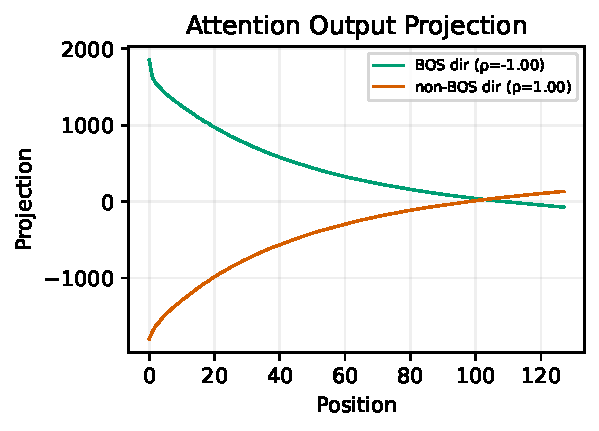
\includegraphics[width=\columnwidth]{plots/r0_attention_output_projection/attention_output_projection_full12h.pdf}
\caption{\textbf{Directional projections (\modelfull).}
Mean projection curves of Layer-2 attention update $\oB{t}$ onto
$\dBOS{2}$ and $\dNBOS{2}$ over $n_{\text{seq}}=320$ held-out sequences at $L=128$.}
\label{fig:gauge_projections_full}
\end{figure}

\begin{figure}[t]
\centering
\begin{subfigure}{0.48\columnwidth}
\centering
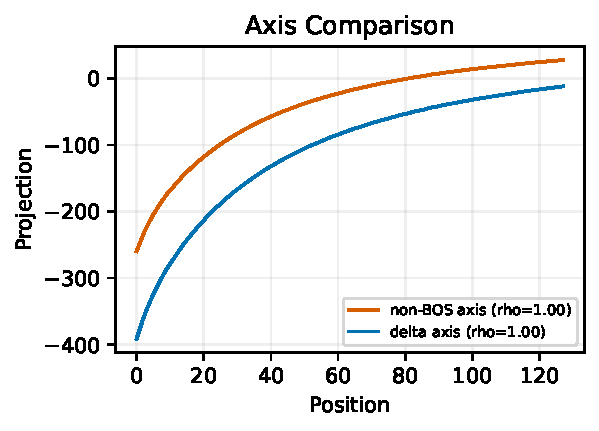
\includegraphics[width=\linewidth]{plots/r0_attention_output_projection/attention_output_axis_compare_attn2_1h.pdf}
\caption{\modelminimal}
\end{subfigure}
\hfill
\begin{subfigure}{0.48\columnwidth}
\centering
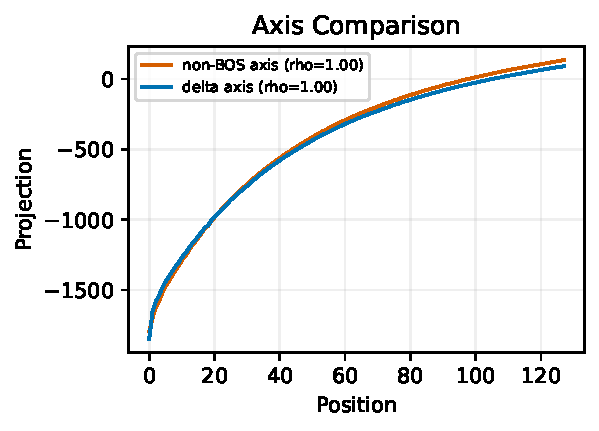
\includegraphics[width=\linewidth]{plots/r0_attention_output_projection/attention_output_axis_compare_full12h.pdf}
\caption{\modelfull}
\end{subfigure}
\caption{\textbf{Axis-comparison projections.}
Mean projection curves of $\oB{t}$ onto $\dNBOS{2}$ and
$d_{\Delta}=(\wNBOS{2}-\wBOS{2})/\|\wNBOS{2}-\wBOS{2}\|$ at $L=128$.
In \modelfull the two axes are nearly equivalent ($\cos=0.984$), while in \modelminimal they are more separated ($\cos=0.764$).}
\label{fig:axis_compare_projection}
\vspace{-3mm}
\end{figure}

\paragraph{Step 5: Head reads the interpolated signal.}
The linear head also aligns with the \nbos direction,
\[
\cos(w_{\text{head}}, \dNBOS{2})=0.319,
\]
and it has weaker alignment with the difference axis,
$\cos(w_{\text{head}}, d_{\Delta})=0.201$.

The weaker alignment ($0.32$ vs.\ $0.73$ in \modelminimal) reflects that \modelfull has additional readout pathways: the trained MLP in Layer~2 can extract position information beyond the pure attention signal, reducing the head's reliance on direct alignment with $\dNBOS{2}$.


\paragraph{Summary.}
Across both \modelminimal and \modelfull, we observe a consistent quantitative signature of the five-step mechanism:
(i) a structural \bos-direction component from causal prefix averaging, (ii) an OV matrix that amplifies and separates \bos vs.\ \nbos directions,
(iii) learned \bos over-attention, (iv) a smooth directional interpolation in the \bos/\nbos plane that tracks position, and (v) a readout aligned with the \nbos direction.

\section{Attention maps \modelfull}
See attention maps figures for \modelfull in \cref{fig:full12h_block1_attention} and \cref{fig:full12h_block2_attention}.
\begin{figure}[h]
\centering
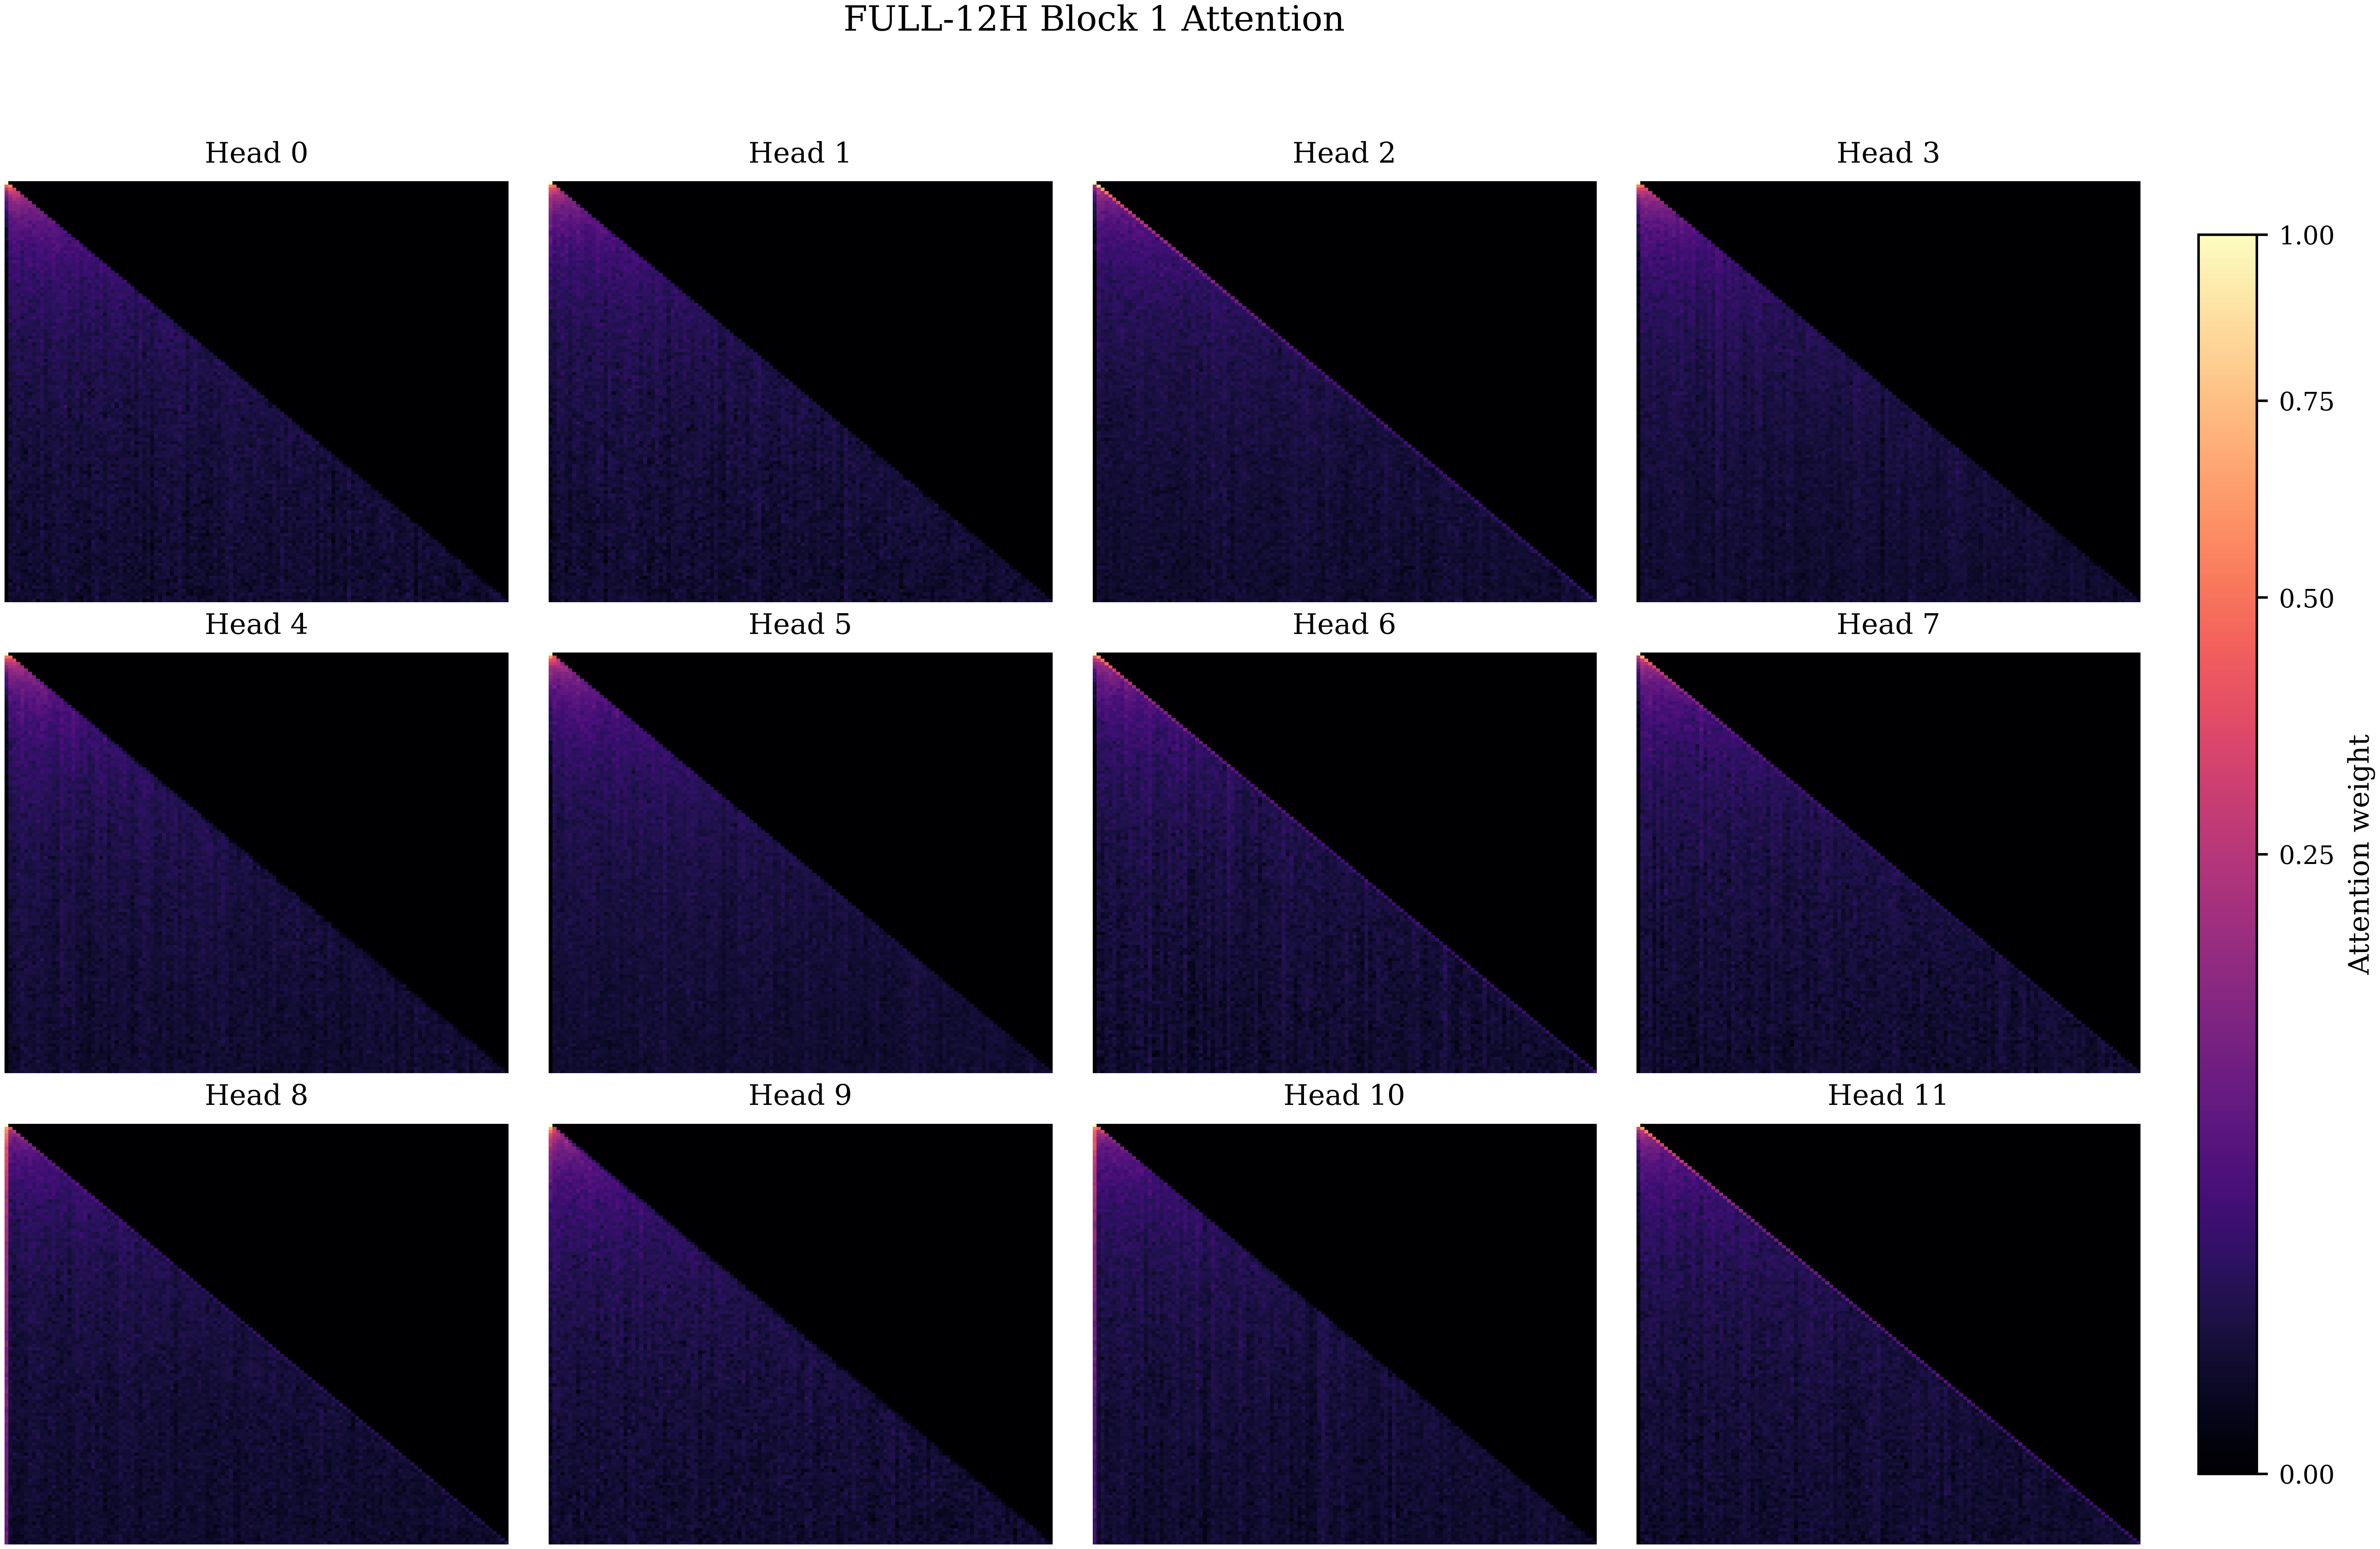
\includegraphics[width=\columnwidth]{plots/attention_uniformity/full12h_block1_attention.png}
\caption{\textbf{\modelfull first-layer attention map.}
Row-normalized mean attention over held-out OpenWebText sequences at $L=128$.}
\label{fig:full12h_block1_attention}
\end{figure}

\begin{figure}[h]
\centering
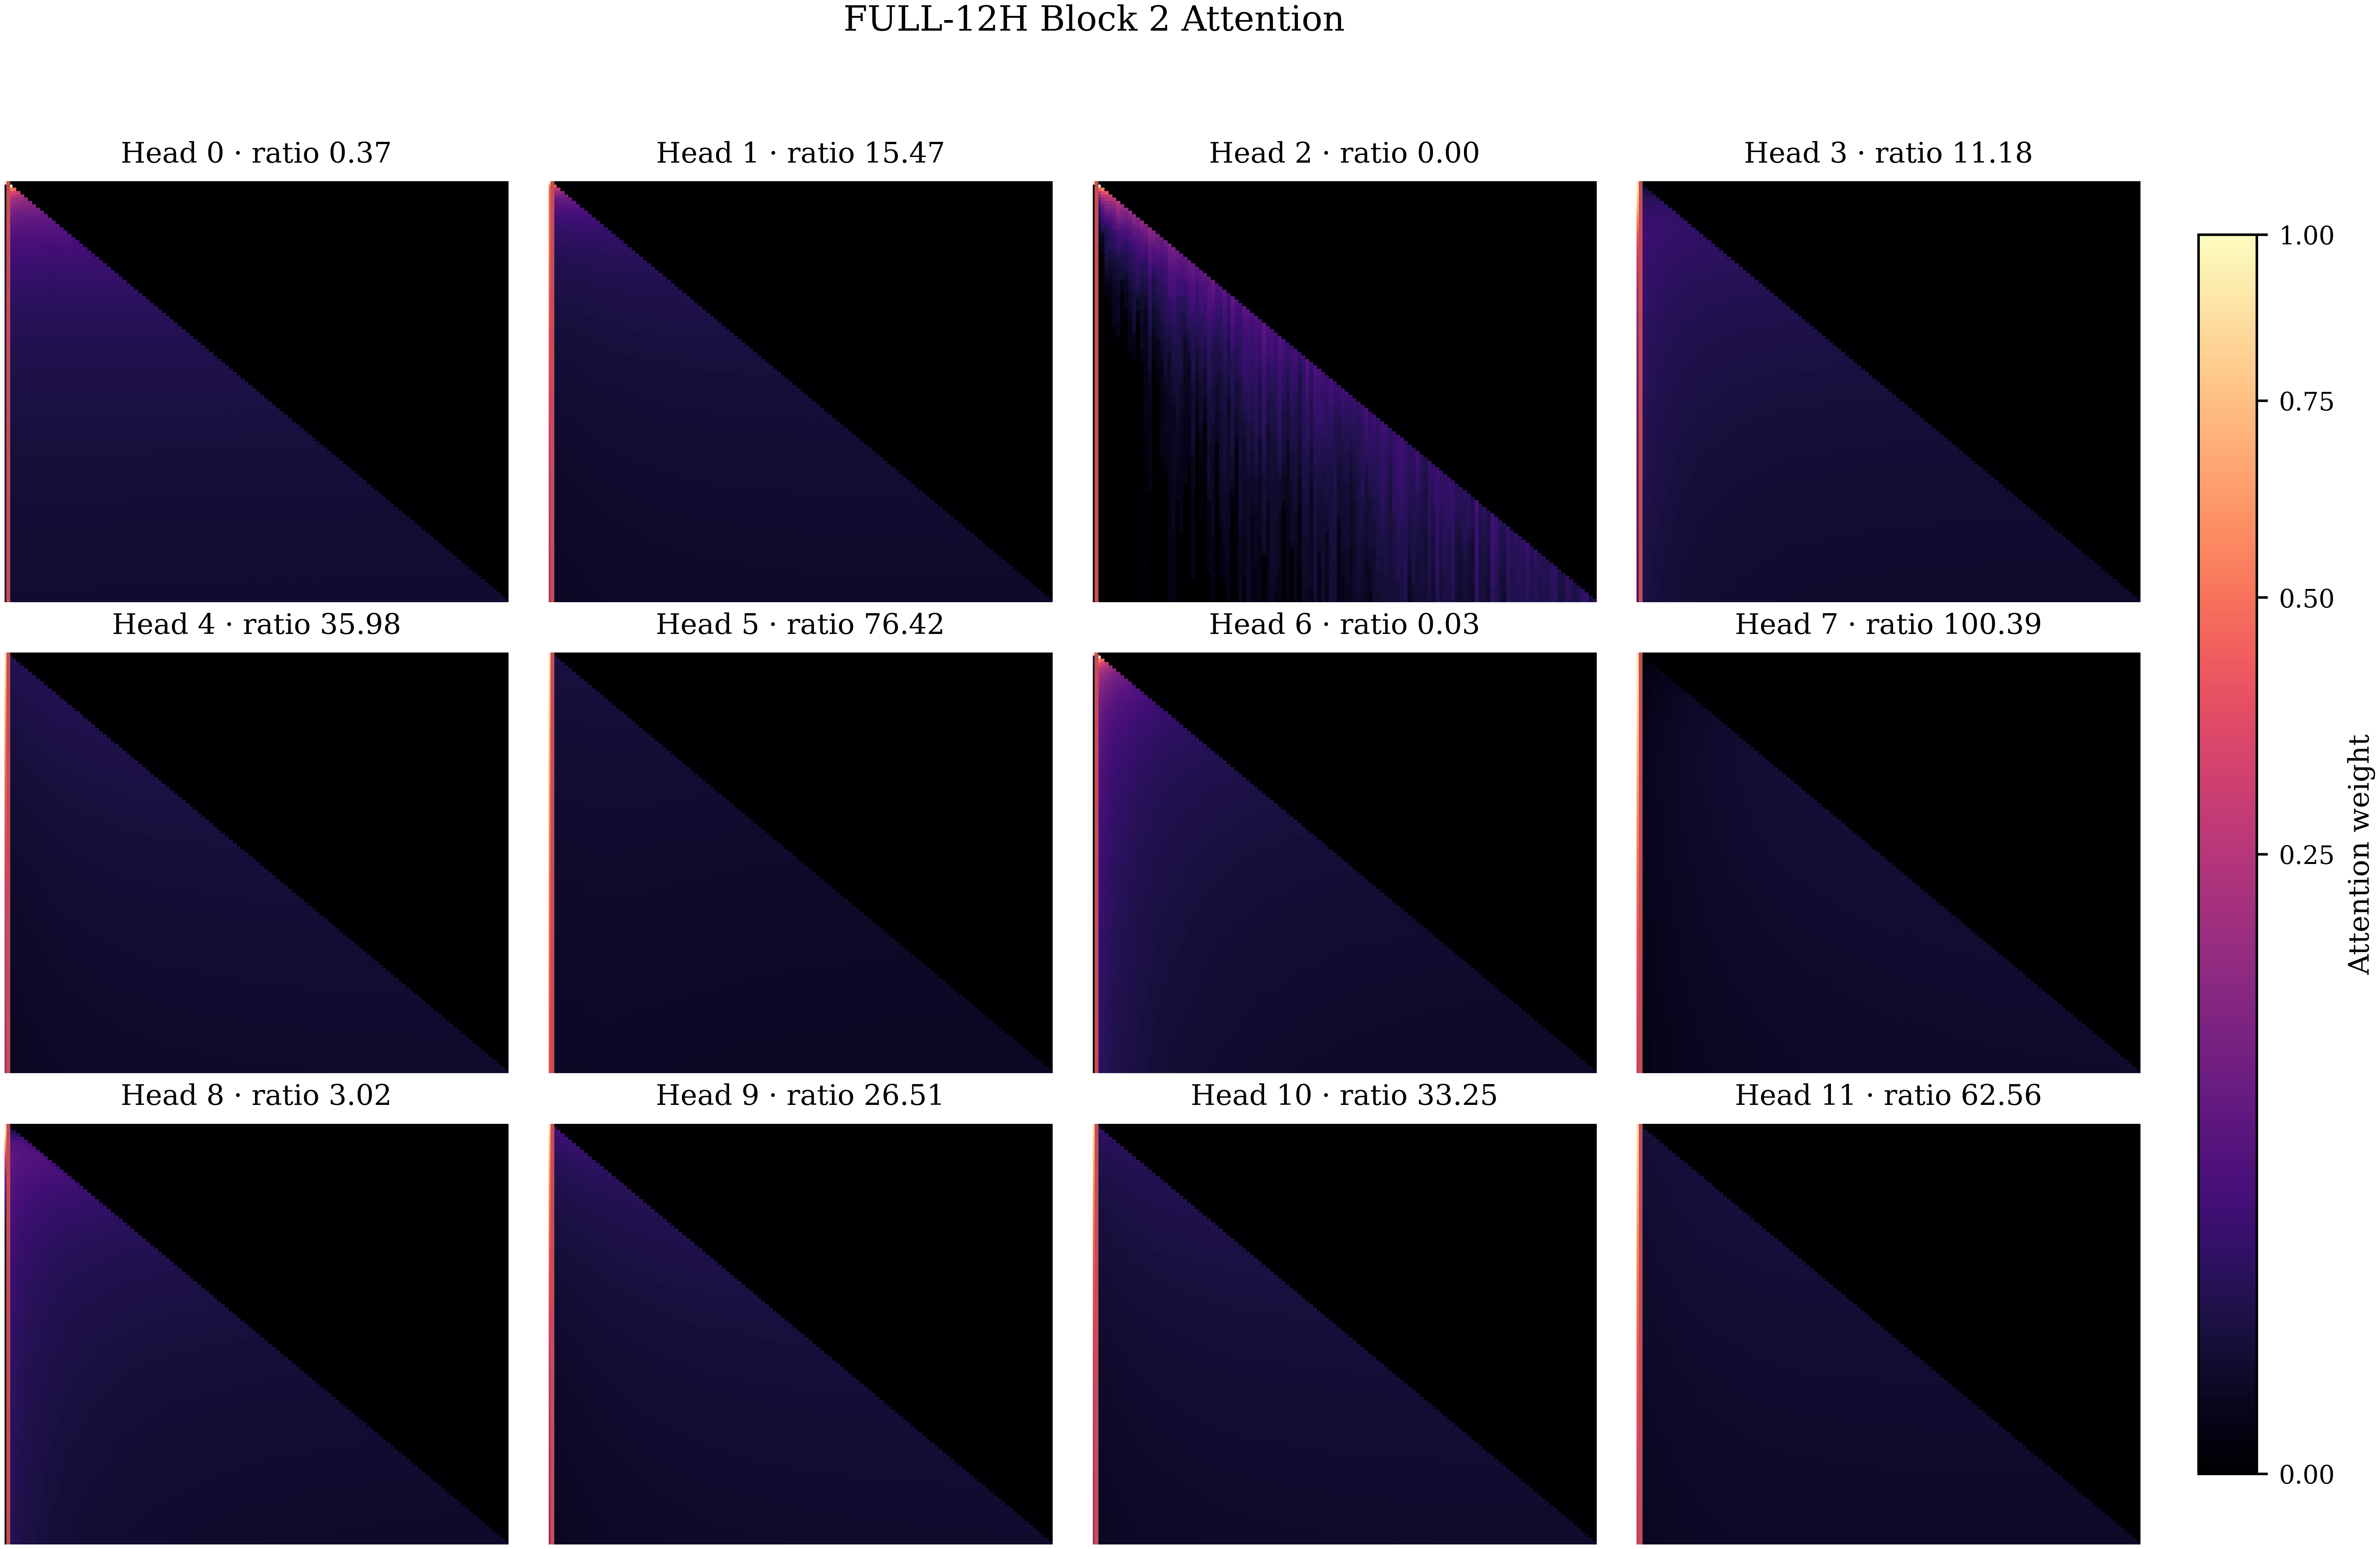
\includegraphics[width=\columnwidth]{plots/attention_uniformity/full12h_block2_attention.png}
\caption{\textbf{\modelfull second-layer attention map.}
Row-normalized mean attention over held-out OpenWebText sequences at $L=128$.}
\label{fig:full12h_block2_attention}
\end{figure}

\section{Directional Trajectory over Individual Sequences}
\begin{figure}[h]
\centering
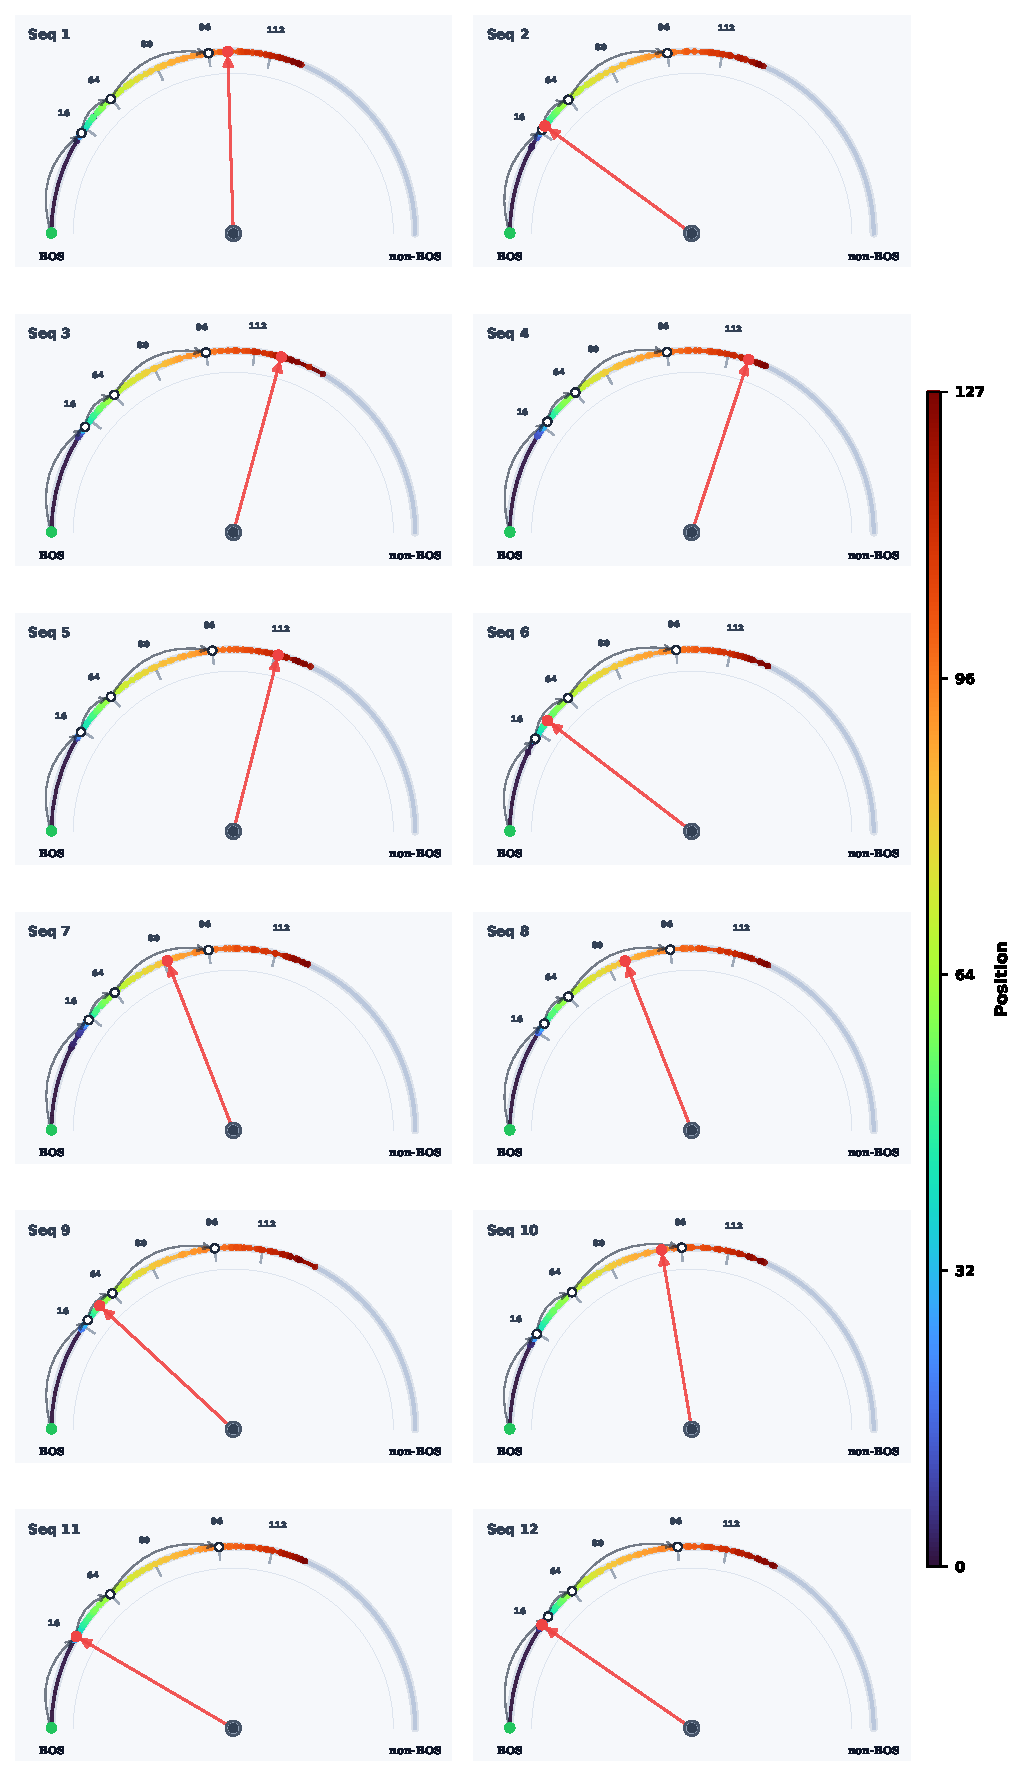
\includegraphics[width=\columnwidth]{plots/r0_directional_rotation_grid.pdf}
\caption{\textbf{Per-sequence directional trajectories in \modelfull.}
Each panel shows one held-out OpenWebText sequence ($L=128$), with no cross-sequence averaging.
The red needle indicates a randomly sampled position in that sequence; despite sample-level variability,
the \bos-to-\nbos directional interpolation is consistently preserved across sequences.}
\label{app:gauge_grid}
\end{figure}

\end{document}
